%! Author = jobdoesburg
%! Date = 04/12/2022

% Preamble
\documentclass[a4paper]{report}

% Packages
\usepackage{hyperref}
\usepackage{url}
\usepackage{graphicx}
\usepackage{parskip}
\usepackage{titling}
\usepackage{a4wide}
\usepackage{caption}
\usepackage{subcaption}

\author{J.J.J. Doesburg}
\title{Remote Document Encryption in SURFfilesender}
\date{\today}

% Document
\begin{document}
    \begin{titlepage}
        \parskip=0pt
        \begin{center}
            \textsc{\LARGE Research Internship Report}\\[1.5cm]

            \begin{minipage}[t]{0.45\textwidth}
                \centering
                
\includegraphics[width=100pt, height=100pt, keepaspectratio]{imgs/logo-ru}\\[0.4cm]
                \vspace{0.4cm}
                \textsc{\Large Radboud University}\\[1cm]
            \end{minipage}
            \begin{minipage}[t]{0.45\textwidth}
                \centering
                
\includegraphics[width=100pt, height=100pt, keepaspectratio]{imgs/logo-surf}\\[0.4cm]
                \vspace{0.4cm}
                \textsc{\Large SURF}\\[1cm]
            \end{minipage}
            \vspace{1.4cm}
            \hrule
            \vspace{0.4cm}
            \textbf{\huge \thetitle}\\[0.4cm]
            \hrule
            \vspace{2cm}
            \begin{minipage}[t]{0.45\textwidth}
                \begin{flushleft} \large
                \textit{Author:}\\
                \theauthor\\
                \texttt{job.doesburg@\{surf,ru\}.nl}\\
                \textit{s4809327}
                \end{flushleft}
            \end{minipage}
            \begin{minipage}[t]{0.45\textwidth}
                \begin{flushright} \large
                \textit{Supervisors SURF:}\\
                William van Santen\\
                \texttt{william.vansanten@surf.nl}\\[0.3cm]
                Nils Vogels\\
                \texttt{nils.vogels@surf.nl}\\[1.3cm]
                \textit{Supervisor RU:}\\
                Bart Mennink\\
                \texttt{b.mennink@cs.ru.nl}
                \end{flushright}
            \end{minipage}
            \vfill
            {\large \thedate}
        \end{center}
    \end{titlepage}


    \begin{abstract}
        In 2017, Verheul~\cite{verheul2017remote} proposed Remote Document Encryption (RDE) as a way to encrypt for a user's e-passport.
        In this report, we discuss the implementation of a prototype for RDE in SURFfilesender, a file transfer service used by SURF based on the open source FileSender project.
        Using RDE, senders can generate a secret key that only the e-passport can retrieve, and use this key to encrypt files, without the need to share any secret data.
        Moreover, the sender can authenticate the document holder based on the existing PKI for e-passports, verifying their identity based on information in the document, without relying on a third party (like SURF).
        We will discuss the prototype architecture and implementation, and the next steps that need to be taken to bring the current prototype to a production-ready state.
        We conclude that RDE is a promising technology that can be used to improve the security of file transfer services, but the proposed architecture can also be used for other applications.
        Due to privacy concerns, however, at SURF, RDE can only be used to its full potential with the latest model of Dutch passports or identity cards (issued after August 2021), which are not yet widely available.
    \end{abstract}

    \tableofcontents

    \chapter{Introduction}\label{ch:introduction}
Filesender applications, such as the popular WeTransfer\footnote{\url{https://wetransfer.com}} or its self-hosted open source alternative FileSender project,\footnote{\url{https://filesender.org}} are a popular way to transfer large amounts of data, removing the file size restrictions of regular email.
Due to their popularity, filesender services are a privacy hotspot, too.
That is, large amounts of possibly privacy-sensitive data are uploaded to these services and a possible security breach at such a service could give adversaries access to the data of numerous users.
To improve privacy, end-to-end encryption is required for services like these.

Implementing end-to-end encryption however comes with the problem of key management.
With symmetric encryption, key management can be problematic as keys need to be shared out-of-band via a different secure channel.
The confidentiality of the transfer then is transferred to the confidentiality of this other channel.
In practice with negligent users, this often results in keys being shared unencrypted via email.
Asymmetric encryption could solve this problem, but the practicalities of properly running a dedicated public key infrastructure or alternative infrastructure (like PGP Web of trust\footnote{\url{https://en.wikipedia.org/wiki/Web_of_trust}}) for this purpose, might be even more problematic.

\section{About SURF}\label{sec:about-surf}
SURF is the Dutch organisation of collaborative educational institutions.
SURF offers ICT services to their members, among which some cloud services such as SURFfilesender, based on the open source FileSender project.
Via SURFfilesender, students and staff from these institutions can share large files (up to 1TB) with each other.
SURF has a high focus on security and privacy and thus does not want to process large amounts of unencrypted data with their service.

\subsection{Current end-to-end encryption in the FileSender project}\label{subsec:current-end-to-end-encryption-in-the-filesender-project}
Currently, the FileSender project does implement end-to-end encryption with symmetric encryption (via passwords and PBKDF2).
When users choose to use this option, they are asked to choose or generate a password.
This password is then used to encrypt the files in browser, before they are uploaded to the server.
When the file upload is complete, the server returns a link that can be shared with the recipient in order to download the files.
The password is not sent to the server, but is expected to be shared out-of-band with the recipient.
When downloading the files, the recipient is required to enter the password, which is then used to decrypt the files in browser again.

This way, though SURF does facilitate the transfer of data for their users, they do not have access to the data itself.
Also, in a way, this could be considered as a form of two-factor authentication, as the files can only be retrieved with access to the download link (sent via email to the user's email box) and with knowledge of the password.
This, in principle, makes the service suitable for transferring privacy-sensitive data.

\subsection{Problems with the current end-to-end encryption}\label{subsec:problems-with-the-current-end-to-end-encryption}
The current end-to-end encryption scheme works well, as long as the password has sufficient entropy and is shared securely with the recipient via a different secure channel.
However, in practice, SURF experiences this is often not the case.
Users often share the password via the same email that contains the download link, or they share it via a second email but to the same email inbox.
This is problematic for multiple reasons.

\begin{enumerate}
    \item The password is sent to the same email inbox as the download link, which means that we do not really have two-factor authentication for the download.
    \item The password is sent in plain text, which means that the password is not protected against eavesdropping.
    \item The recipient is made responsible for the secure handling of the password.
\end{enumerate}

Considering these problems, though the current end-to-end encryption scheme works good in theory, in practice it is not sufficient for SURF to be able to offer a service that is suitable for transferring privacy-sensitive data.
Given this situation, SURF is looking for a solution that allows them to provide end-to-end encryption for their users, without the need for the users to share the password out-of-band, guaranteeing this 2FA-like behaviour.

\section{Remote Document Encryption}\label{sec:remote-document-encryption}
In 2017, Verheul proposed Remote Document Encryption (RDE) as a scheme for `encrypting data for e-passport holders'~\cite{verheul2017remote}.
E-passports are passports that contain a chip implementing the ICAO 9303 standard~\cite{icao9303securitymechanisms}.
We immediately note that although only passports implement this standard, also other documents, like national ID cards and drivers licenses, implement significant parts of this standard and can thus be used as well.
In the rest of this report, we will use the term e-passport, passport, or document interchangeably to refer to these documents, unless otherwise specified.
The RDE scheme is based on the idea that the e-passport can be used as a wireless HSM (Hardware Security Module), generating symmetric keys (shared secrets with some other party) that can be used for encryption.
In this terminology, we consider \textit{recipients} as the document holders, and \textit{senders} as the parties that want to send data to the recipients in an encrypted way.

\subsection{RDE scheme in short}\label{subsec:rde-scheme-in-short}
Recipients in this scheme first need to register their e-passport for usage with RDE at some database.
During enrollment, some data from the e-passport is extracted.
These are called enrollment parameters and one could consider them as the RDE public key of the e-passport (though we will not use the word `public key' as to avoid confusion later on).
Senders can then, based on this public key, generate a secret key that is shared between them and the e-passport, together with so-called decryption parameters.
The passport holder can use these decryption parameters, together with their e-passport to retrieve the secret key.
The decryption parameters here do not need to stay secret, as they are only used to retrieve the shared secret from the e-passport.
A very simplified version of the RDE scheme is shown in Figure~\ref{fig:rde-scheme-very-simple}.
\begin{figure}
    \centering
    
\includegraphics[width=0.8\textwidth]{imgs/RDE very simple}
    \caption{Simplified version of the RDE scheme.}
    \label{fig:rde-scheme-very-simple}
\end{figure}

\subsection{Authenticating the e-passport holder}\label{subsec:authenticating-the-e-passport-holder}
In its most basic form, the RDE scheme does not authenticate the e-passport holder.
The passport here just serves as an HSM (Hardware Security Module) that can output a key based on some input.
This already makes the scheme suitable for end-to-end encryption, as the sender and the recipient can use the key to encrypt and decrypt the data without actually having to share the key with each other.
However, the RDE scheme can be extended to also authenticate the e-passport holder using the government PKI (Public Key Infrastructure) that is used for e-passports.

In 2020, Verheul further described a secure filesender service based on RDE, where the e-passport holder is authenticated using the existing PKI for e-passports~\cite{verheul2020secure}.
During registration, additional data is extracted from the e-passport, which is used to authenticate the e-passport holder.
This includes for example the name, nationality and date of birth of the e-passport holder, but could also include other data, such as the facial image of the e-passport holder.

\section{SURFfilesender with RDE}\label{sec:surf-filesender-with-rde}
In this report, we describe how the SURFfilesender (or actually, the FileSender project) can be extended with RDE to provide end-to-end encryption for their users, without the need for the users to share the password out-of-band.
We describe an infrastructure for using RDE in applications, where we specifically focus on the SURFfilesender.
The infrastructure, however, can be used for other applications as well.

For this prototype, a number of components have been developed, which are described in the following sections.
Some components form the basis of the RDE scheme, while others are specific to the SURFfilesender application.
Especially the latter ones are not meant to be used in a production environment, but are only meant to be used as a proof-of-concept to demonstrate the feasibility of the proposed solution.
Most notably, our prototype does not implement protection against, for example, phishing attacks, denial of service attacks, or active MITM attacks on parts of the protocol that do not involve RDE itself.
We consider the challenge to implement such protections to be very much feasible, but out of scope for this report.

A proof-of-concept walk-through of in-browser RDE is available at \url{https://demo.rde.filesenderbeta.surf.nl} and the source code is available at \url{TODO}.

\subsection{Alterations to the original secure filesender proposal}\label{subsec:alterations-to-the-rde-scheme}
Verheul already described a secure filesender service based on RDE, where the e-passport holder is authenticated using the existing PKI for e-passports~\cite{verheul2020secure}.
Though the name suggests differently, the term `filesender service' in his paper does not refer to the actual FileSender project, but to a generic filesender service.
The focus of this paper is on the SURFfilesender specifically.

Though the general outline of the RDE scheme in our report is the same, the implementation we describe in this report is notably different from the proposal in~\cite{verheul2020secure} and more closely follows the original RDE scheme as described in~\cite{verheul2017remote}.

The main reason for this is that the open source FileSender project already has end-to-end encryption implemented, which we can use as a basis for our implementation.
We thus only use the key agreement part of the scheme, and use the existing end-to-end encryption implementation of the FileSender project for the actual encryption of the files.

Moreover, we take a different approach to the authentication of the e-passport holder, because the proposal by Verheul is not compatible with SURF's way of operating.
Our more naive approach does not require any trust in SURF for authentication of users, and does not require SURF to process any sensitive data that may not be revealed to others.
This does come at the cost of less privacy for the e-passport holders, but with recent developments with Dutch e-passports, this may not be a problem anymore.

\subsection{Benefits of the proposed solution}\label{subsec:benefits-of-the-proposed-solution}
The proposed solution has a number of benefits over the current (password-based) end-to-end encryption scheme of the FileSender project.

\subsubsection{True end-to-end encryption}\label{subsubsec:true-end-to-end-encryption}
First of all, the proposed solution does not require the users to share a password out-of-band.
Instead, the encryption key is retrieved from the e-passport and never sent over a network (in unencrypted form).
Consequently, the proposed solution provides 2FA-like functionality for the download of the file: the recipient of a file transfer needs to both know the download link (that is unique and should only be sent to the recipient obviously) and be in possession of the e-passport in order to retrieve the files.

\subsubsection{'People already have an e-passport'}\label{subsubsec:people-already-have-an-e-passport}
The aforementioned benefits, however, are not specific to the usage of RDE with e-passports.
In fact, the same benefits can be achieved by using any other HSM, such as a Yubikey, or even a smartphone.

An additional advantage of using an e-passport is that they are already widely available (`everybody has one'\footnote{
    It is a huge misconception that everyone in the world has a passport or national identity card.
    Even within the Netherlands, it is technically not mandatory to have one, only when you are somewhere in public space.
    Generally, though, and especially in Europe, it is very common to own such a document.
}), and that they are already used for authentication purposes.
For organisations like SURF and its members, this means that there are no additional costs involved in the usage of end-to-end encryption.

Another advantage is that, in contrast to using commercial HSM devices, users have an intrinsic interest in keeping their passport secure.
People are unlikely to share their passport with others or leave it somewhere unattended, as this could lead to the passport being stolen or lost and possible identity theft.
We expect people to handle their passport more securely than any commercial HSM device.
Generally, at least in the Netherlands, people are more likely to always have their identity documents with them, while commercial HSM devices or even phones might not be available at all times.

\subsubsection{Use existing governmental PKI}\label{subsubsec:use-existing-governmental-pki}
Moreover, using e-passports comes with the additional benefit that the e-passport holder can be authenticated using the existing PKI for e-passports run by governments.
Specifically for SURF, this means that SURF does not need to be responsible for the authentication of the recipient.
This is done via the government.
This is especially important as the recipients of the SURFfilesender are not necessarily affiliated with SURF itself (but with its members).
This means that SURF cannot be making claims about their identity themselves, as it does not know them directly.

    \chapter{Basic RDE Scheme}
\label{ch:basic-rde-scheme}

In this chapter we further explain the basic RDE scheme presented in~\cite{verheul2017remote}.

We distinguish three phases in the RDE scheme: (1) enrollment, (2) key generation, and (3) decryption (or key retrieval).
In the enrollment phase, the user (recipient) enrolls their passport for usage with RDE by extracting some data from the passport.
This is done by using a reader app that can communicate with the passport via NFC.
Enrollment results in certain \textit{enrollment parameters}, which one could consider as some sort of RDE public key of the user.
We will however not use the term public key further, as this could be confusing with actual the public key of the password that is included in the enrollment data.
We rather use the term \textit{enrollment parameters}.

In the key generation phase, someone (the sender) retrieves the \textit{enrollment parameters} and generates an RDE key pair for the recipient.
This results in a \textit{secret key}, and \textit{decryption parameters}.
The \textit{secret key} can be used to do the actual encryption of the message or files.
The \textit{decryption parameters} need to be sent back to the recipient, together with the encrypted message or files and does not need to be kept secret.
During decryption, the recipient uses the \textit{decryption parameters} together with their passport to retrieve the secret key and actually decrypt the message or files.

A high-level overview of this scheme is shown in Figure~\ref{fig:basic-rde-scheme}.
\begin{figure}
\centering

\includegraphics[width=0.8\textwidth]{imgs/RDE overview}
\caption{High-level overview of the basic RDE scheme.}
\label{fig:basic-rde-scheme}
\end{figure}

\section{E-passports}
\label{sec:e-passports}
E-passports are electronic passports that function as a smart card.
They contain a chip that can store data and execute programs.
Data on e-passports is stored in files, called Elementary Files (EFs) containing certain Data Groups (DGs).
For our report the most interesting files on the passport for RDE are the DG1, DG2, DG14, and EFsod.
\begin{itemize}
    \item DG1 contains the personal data of the holder of the passport.
    This group contains the information that is also printed on the passport itself in the machine-readable zone (MRZ).
    The data in this group is thus also referred to as the MRZ data.
    \item DG2 contains the facial image of the holder of the passport.
    \item DG14 contains security info of the passport.
    Most notably, it contains the Chip Authentication (CA) public key of the passport
    \item The EFsod contains the security object data of the passport.
    It contains a hash of all data groups on the passport, as well as a certificate from the country that issued the passport.
    The certificate can be used to verify the authenticity of the data.
\end{itemize}

\subsection{Secure messaging (BAC and PACE)}\label{subsec:secure-messaging}
Readers can communicate with an e-passport at different levels of security.
The most basic level is plain messaging and does not provide any security features.
At this level, the passport will not respond to any commands, except for querying the supported security levels and initiating a secure messaging session.
In order to actually communicate with the passport, a secure messaging channel must be set up.
Currently, there are two ways to set up a secure messaging channel: Basic Access Control (BAC) and Password Authenticated Connection Establishment (PACE).

\subsubsection{Basic Access Control (BAC)}\label{subsubsec:basic-access-control}
BAC works via a challenge response mechanism, where the reader requests a random challenge from the passport, and then shows knowledge of the BAC key by properly responding to this challenge.
The key is based on three fields from the MRZ: the date of birth, the date of expiry, and the document number.
After BAC, further communication with the passport is encrypted using the 3DES algorithm.

\subsubsection{Password Authenticated Connection Establishment (PACE)}\label{subsubsec:password-authenticated-connection-establishment}
A second and more modern way for this first level of security is Password Authenticated Connection Establishment (PACE).
PACE first performs a (Elliptic Curve) Diffie-Hellman key exchange to generate a session key, which is then used to encrypt the communication.
Authentication is then still done with the BAC key derived from the MRZ data (or on certain passports, with the Card Access Number (CAN) that is printed on the passport).
According to the ICAO standard, PACE is the preferred method for setting up a secure messaging channel as it is more secure than BAC.
BAC should only be used as fallback when PACE is not supported by the passport~\cite{icao9303securitymechanisms}.
Note that on the most recent Dutch passports, BAC is no longer supported and PACE must be used for the first level of security.


BAC and PACE do not provide any real authentication of the document itself or the document holder.
They only prevent eavesdropping on the communication between the reader and the passport and prevent skimming attacks (where an attacker reads data from the passport without the user noticing, for example when walking through an airport).
Using the BAC key (or CAN) requires the reader of the passport to actually have physical access to the passport (or at least the MRZ data).

\subsection{Passive Authentication (PA)}\label{subsec:passive-authentication}
After the first level of security has been established, the reader can read data from the document.
To authenticate whether this data actually belongs to a valid passport, the reader can perform passive authentication.
This requires the contents of the EFsod file to be read from the passport.
The reader can calculate the hashes of the data groups on the passport and compare them to the hashes in the EFsod file.
Additionally, it should verify the authenticity of the read EFsod file by checking a hash on those contents, and verifying the signature on the file.
This signature is created using the public key of the country that issued the passport, the so-called \textit{document signing key}.
Finally, the certificate chain should be verified.
This ultimately requires the reader to have a trusted list of document signing keys.
There are several ways to obtain such list, for example by downloading it from the ICAO website, or from a country's public key directory.

Note that the steps above are all be performed by the reader and do not require any processing capabilities on the passport itself.
This is why these steps are called passive authentication: the passport does not actively participate in the authentication process.

\subsection{Chip Authentication (CA)}\label{subsec:chip-authentication}
The aforementioned passive authentication only verifies the authenticity of data on the passport, but does not verify if the data is actually from the physical passport that is presented.
We could also be dealing with a fake passport that is replaying the data from a real passport.
In order to verify that the passport is actually the passport that is presented, the passport needs to actively participate in an authentication protocol.
This can be done via different protocols: by Active Authentication (AA) or Chip Authentication (CA).
For RDE, we use only use the latter.

Chip Authentication (CA) is a protocol that uses the CA public key of the passport to authenticate the passport.
This key is stored in the DG14 file on the passport.
Upon perform CA, (Elliptic Curve) Diffie-Hellman is performed between the passport and the reader.
The shared secret of this handshake is then used for further communication in the session.
Note that this replaces the keys that were set up earlier with BAC or PACE.

Note that with CA, the passport proofs it has access to the private key that belongs to the CA public key (which in its turn is signed by the government via the EFsod).
This is how we know that we are communicating with the real passport and not a fake passport that is replaying.

Note that according to the ICAO standards, CA does not necessarily need to be ECDH, but can also be RSA-based.
However, in practice, ECDH is used more often.
We will use the term ECDH in the rest of this report, but note that RSA-based DH also works.

\subsection{Terminal Authentication (TA)}\label{subsec:terminal-authentication}
For completeness, we also briefly mention Terminal Authentication (TA).
With TA, the reader proves to the passport that it is a trusted reader, via a challenge-response mechanism.
This is required for some applications.
For example, in order to read certain biometric data from the passport, like fingerprints, the reader must prove to the passport that it is a trusted reader.
For RDE, we do not use TA.

\section{RDE basic idea}\label{sec:rde-basic-idea}
When performing the CA ECDH key exchange step, the passport will always use the same key for its part of the handshake: it uses the public key that is stored in the DG14 file.
After CA, further communication is encrypted using keys deterministically derived from the shared secret of the ECDH key exchange.
This means that the freshness of the communication, relies on the freshness of the ephemeral key chosen by the reader.

After CA, when the reader tries to read the data on the passport, the passport will respond with a ciphertext that is encrypted using the keys derived from the shared secret.
Because strong encryption is used, the data will look random to anyone not in possession of this shared secret.
Everytime a reader chooses the same ephemeral key for its part in the ECDH key exchange, the same shared secret will be generated, and reading this data group will result in the same ciphertext.
RDE is based on this idea.

\begin{enumerate}
    \item Upon enrollment, we read the CA public key of the passport (after having performed BAC or PACE).
    We also read the contents of one of the data groups on the passport.
    This can be any data group that can be read without TA.
    In most cases, this will be DG14 as this data group does not contain any privacy-sensitive data and is of sufficient size to return long enough ciphertexts later.
    \item During RDE key generation, we retrieve this information and choose our own ephemeral key that is compatible with the CA public key of the passport.
    We simulate ECDH with the CA public key of the passport (that is included in the enrollment parameters) and compute the shared secret.
    We then use this shared secret and the derived keys to emulate how the passport would reply to us when we would try to read the contents of the chosen data group (from which we know the plaintext from the enrollment parameters).
    This emulated ciphertext response will be used to construct the secret key.
    Furthermore, we also need to emulate, using the shared secret and the derived keys, what our encrypted read command should look like if we were to actually communicate with the passport.
    The emulated encrypted read command (also referred to as protected command), together with the public key we chose ourselves, together form the RDE decryption parameters.
    \item When as recipient, we want to retrieve the secret message key, we use the provided RDE decryption parameters.
    First we perform BAC or PACE to set up the first level of security.
    Then we perform the ECDH with the provided public key from decryption parameters (that was chosen by the sender).
    Even though we as recipient do not know the shared secret our passport is using (as we do not have the private key the sender generated), the passport will know this shared secret (as it is based on the private key that is securely stored on the passport).
    We then send the protected command to the passport.
    The passport will be able to decrypt this command, and then reply with the encrypted contents of the chosen data group.
    This will match the ciphertext response that was emulated by the sender.
    The reader then derives the secret key from this ciphertext response.
\end{enumerate}

For deriving the secret key from the ciphertext response, we simply take a hash of the ciphertext.

For further details on the RDE protocol, we refer to the explanation provided in~\cite{verheul2017remote}.
A schematic of the decryption process is shown in Figure~\ref{fig:rde-decryption}.
\begin{figure}
    \centering
    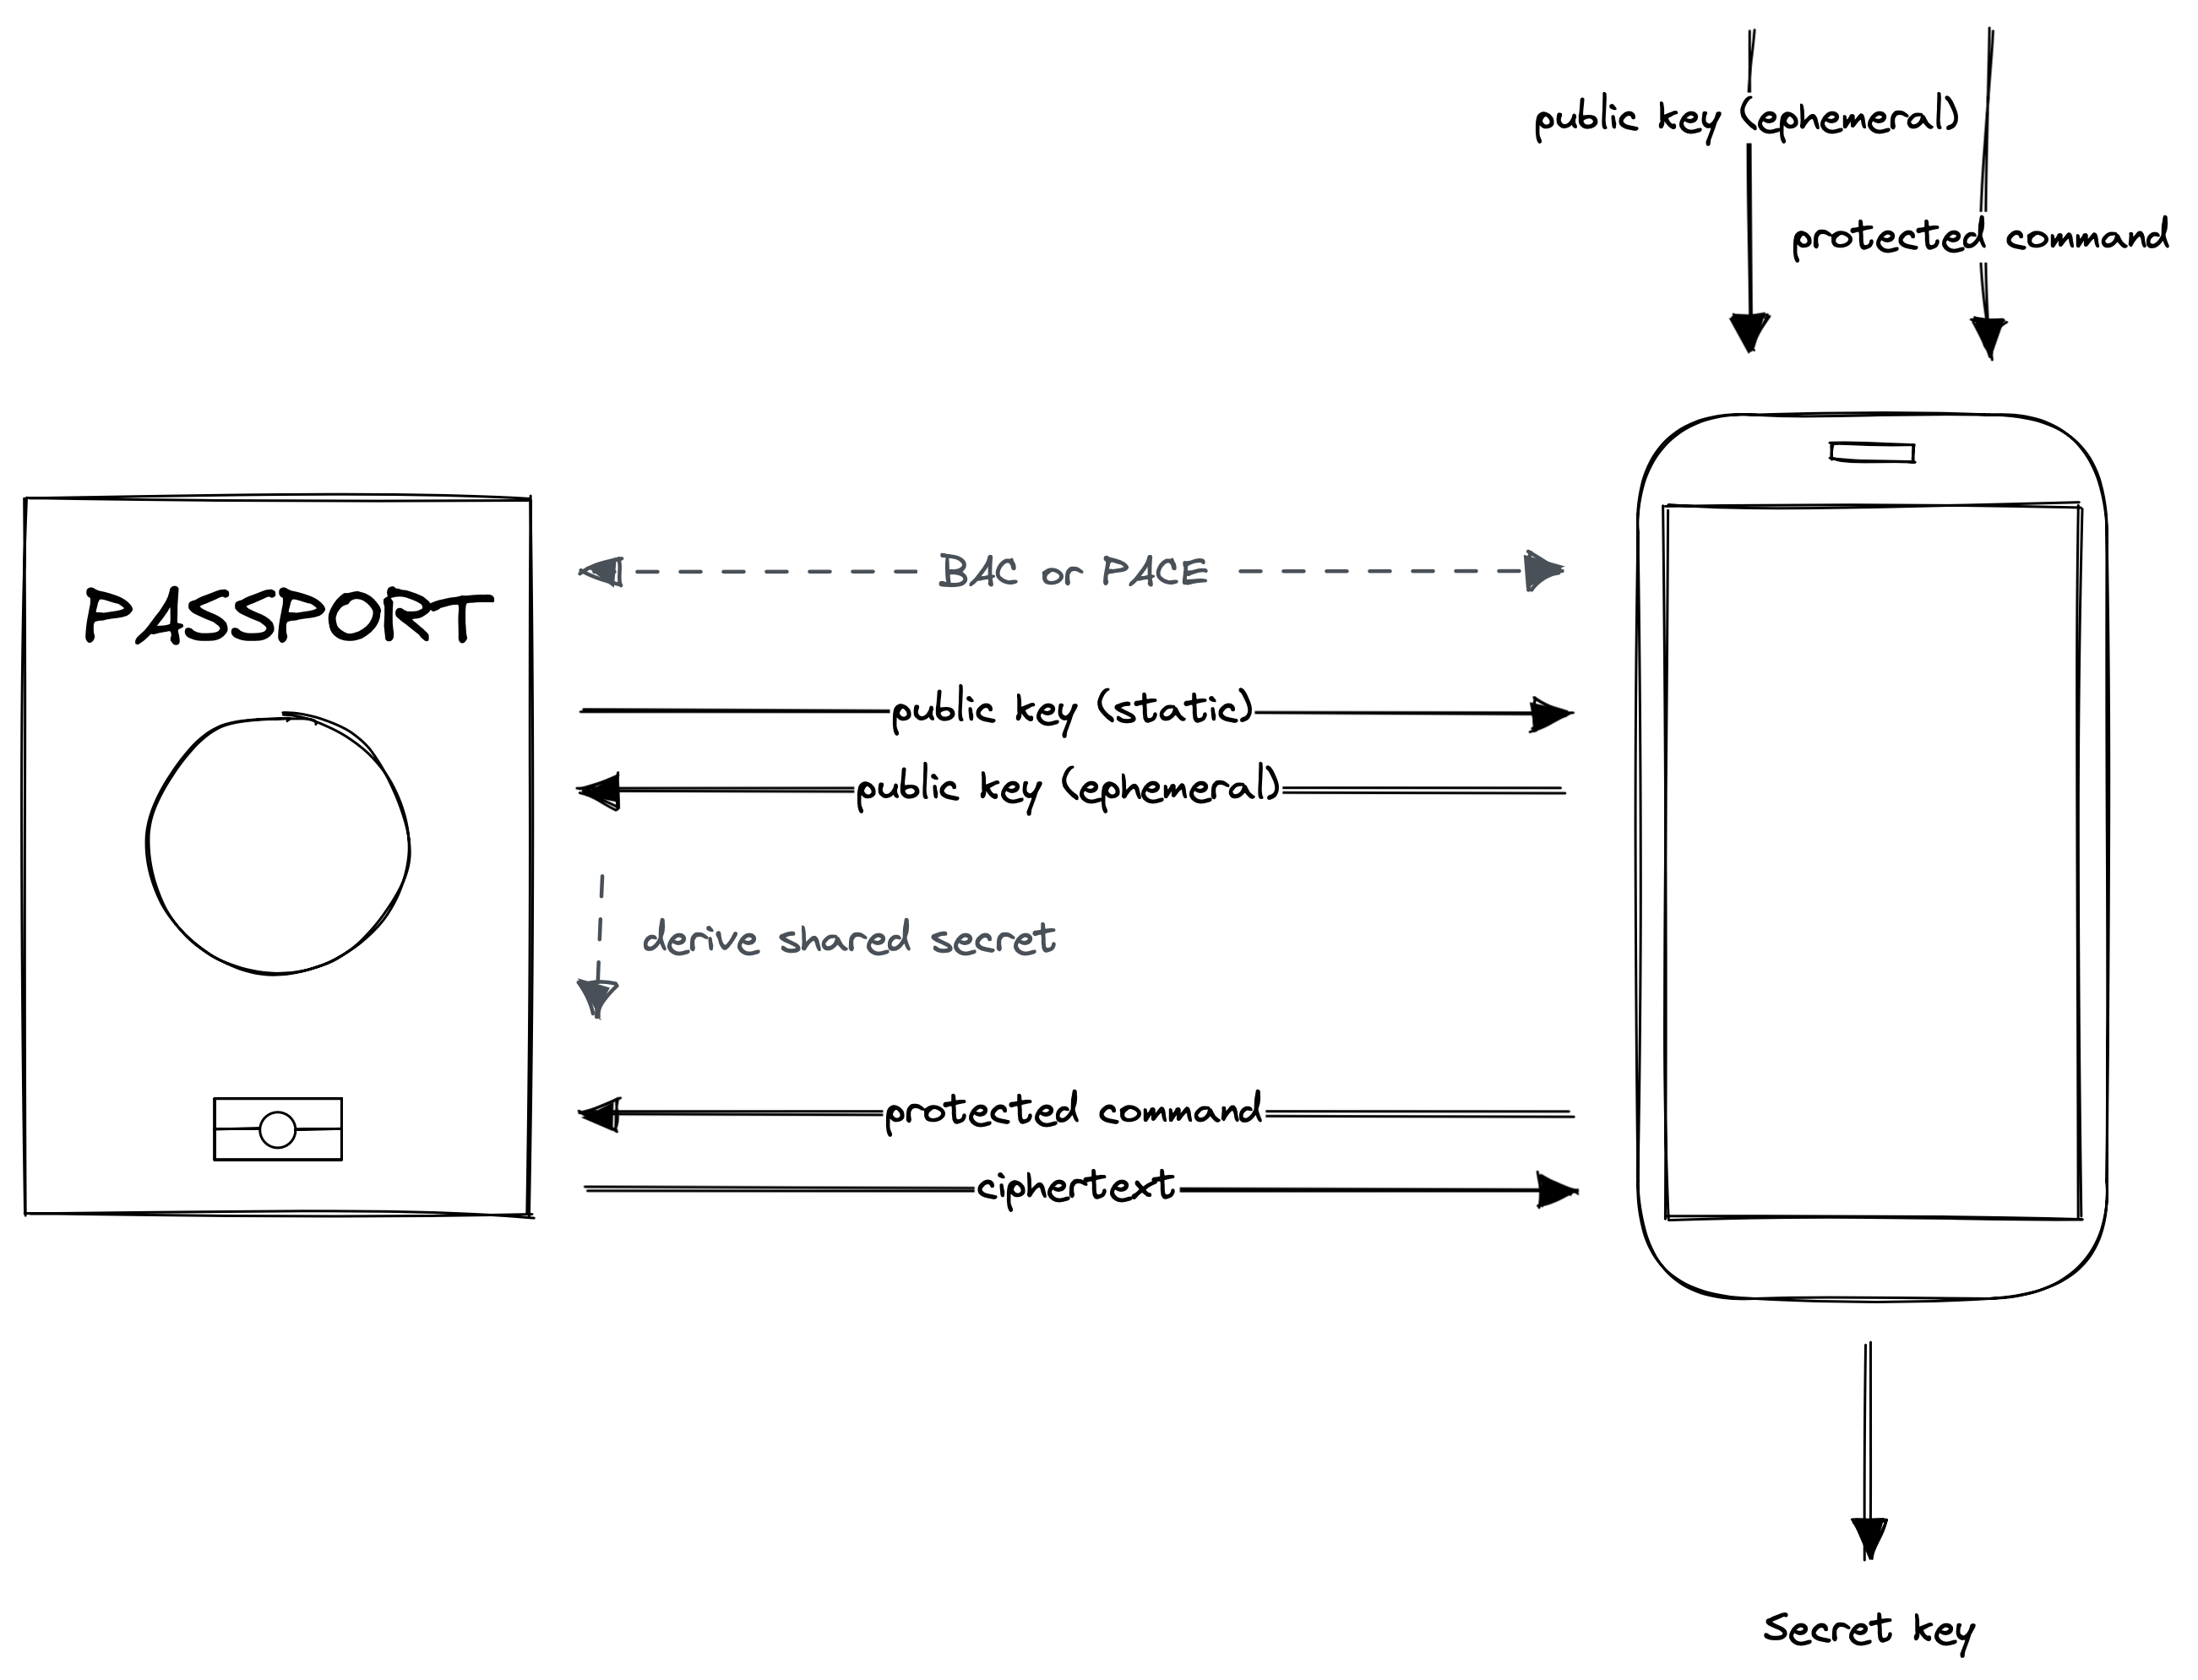
\includegraphics[width=0.8\linewidth]{imgs/RDE decryption}
    \caption{RDE decryption process}
    \label{fig:rde-decryption}
\end{figure}

\subsection{Trusting the reader}\label{subsec:trusting-the-reader}
We note that the reader itself does not store any secret information.
It only interfaces with the passport.
During the decryption (key retrieval) process, however, the reader will receive the secret key.
More importantly, the ciphertext that is used to derive the secret key is sent `in the clear' from the passport to the reader.
This means that not only the reader, but also anyone eavesdropping the communication between the reader and the passport can read this ciphertext.
For normal communication with the passport, BAC (though weak) or PACE offers protection against eavesdropping.
After CA, however, this protection is replaced.
For decryption, we thus need to trust the reader and the environment in which the reader is used.

\section{ICAO compatibility}\label{sec:icao-compatibility}
The RDE protocol relies on e-passports being able to perform Chip Authentication (CA) according to the ICAO standards~\cite{icao9303securitymechanisms}.
There are different key exchange protocols and cipher algorithms that can be used for CA.

The ICAO standard describes both standard RSA based Diffie-Hellman key agreement (DH) and ECDH based Diffie-Hellman key agreement (ECDH)~\cite{icao9303securitymechanisms}.
The standard also specifies that further communication should be encrypted using 112 bit 3DES in CBC mode, or 128-bit AES in CBC mode with CMAC, or 192-bit AES in CBC mode with CMAC or 256-bit AES in CBC mode with CMAC.
The standard does not restrict the use of specific curves for ECDH, meaning that any curve can be used.
However, it does specify a number of standard curves that can be used:
\begin{itemize}
    \item \texttt{brainpoolP192r1}
    \item \texttt{brainpoolP224r1}
    \item \texttt{brainpoolP256r1}
    \item \texttt{brainpoolP320r1}
    \item \texttt{brainpoolP384r1}
    \item \texttt{brainpoolP512r1}
    \item \texttt{secp192r1}
    \item \texttt{secp224r1}
    \item \texttt{secp256r1}
    \item \texttt{secp384r1}
    \item \texttt{secp521r1}
\end{itemize}
Any e-passport that is compliant with the ICAO standard on this level should be able to perform RDE.

As noted by Verheul in~\cite{verheul2017remote}, also other national ID cards and electronic drivers licenses that implement the ICAO CA(v1) standard should be able to perform RDE.
German identity cards, however, do not implement the ICAO CA v1 standard, but rather uses CA v2 that is not compatible with RDE because no static key from the passport is used in the key exchange.
Moreover, the German identity card requires the use of TA before reading any data group.

\section{Security}
\label{sec:security}
As described in~\cite{verheul2017remote}, the security of RDE is based on the security of the underlying CA protocol and the security of the encryption used for further communication.
For the Brainpool320r1 curve with 256-bit AES in CBC mode with CMAC, used on Dutch documents, RDE gives us 160-bit security.
Verheul does describe how longer ciphertexts can be achieved by not using a single protected command, but by using multiple protected commands, reading more bytes from data groups.
In this report, we do not go into the details of this, nor did we implement this, as the 160 bit security is already sufficient for our use case.

    \chapter{RDE with document holder authentication}\label{ch:rde-with-document-holder-authentication}

As mentioned earlier, the RDE scheme presented in~\cite{verheul2017remote} in its most basic form does not provide any authentication of the document holder.
In this chapter we will explain how to add document holder authentication to the basic RDE scheme.
This concept has already been presented in~\cite{verheul2020secure}.
Our implementation, however, is different from the one presented in~\cite{verheul2020secure}.
In this chapter, we will first elaborate on our implementation and then explain the differences.

While the developed infrastructure will only be presented in the next chapter, we will already use the concept of a key server in this chapter.
The key server is a partially trusted party that is responsible for storing the enrollment data of users (recipients).
Senders can query the key server for the enrollment data for a recipient, for example based on the recipient's email address.
Because the email address is not contained in the e-passport, the key server needs to verify the email address of the sender.
As we will see, however, we do not need to further trust the key server for other claims on the user's identity, following our implementation.

\section{RDE \textit{without} document holder authentication}\label{sec:rde-without-document-holder-authentication}
The RDE scheme described before does provide us with the ability to generate a shared secret key between the sender and the receiver.
However, as sender, you do not know if the receiver is the actual document holder.
Upon requesting the enrollment data for a receiver from the keyserver, you do not have the ability to verify that this enrollment data actually belongs to the receiver, other than trusting the key server.
The user could be using the passport of another user, for example, a passport that has expired or revoked by a government (possibly because it does not offer sufficient security), or even use an especially crafted fake passport of which copies can exist.

This could give unfair security assumptions to the sender.
In daily life, passports are primarily a means of identification and authentication.
Any sender might thus falsely assume that with using RDE, the key server verified that the recipient is who they claim to be, while this is not the case.

\section{Adding document holder authentication}\label{sec:adding-document-holder-authentication}
Adding extra information about the document holder to the enrollment data turns out to be easy.
Upon enrollment, we should not only extract the contents of the data group we want to use for RDE, but also the contents of the data group that contains the document holder's personal data.
Most notably, this could be DG1, but it might also be interesting to include DG2, that includes the document holder's facial image.
The enrollment data should then be extended to also contain the contents of these data groups.
Most importantly, we should include the contents of EFsod.
With this information, anyone can perform passive authentication, as mentioned in section~\ref{subsec:passive-authentication} (checking hashes, signature, and certificate chain).
This means that any party, including the key server itself, can verify that the enrollment data belongs to the actual document holder at any time.
Because in RDE, Chip Authentication is performed, we also know that on decryption, the document actively authenticates itself too.

This way, we do not only have the ability to generate a shared secret key between the sender and the receiver, but we immediately verify the document holder's identity via the governmental PKI.
Because the RDE data group is bound to this information, this essentially guarantees that only the document holder (of anyone in possession of their document) can retrieve the secret key.
Note that we can also check if the document has expired or been revoked by the government, as we can check the validity of the certificate chain.

Following this approach leads basically to 4 levels of overall RDE security:
\begin{enumerate}
    \item \textbf{Basic RDE}:
    The sender and receiver can generate a shared secret, but the sender does not have any guarantee on the integrity of the receiver's document or identity.
    They could be using a fake, expired, or insecure document or a document of another person.
    We fully trust the key server to provide us with the correct enrollment data for the receiver.
    \item \textbf{RDE with EFsod}:
    The sender and receiver can generate a shared secret, and the sender can verify that the receiver uses a valid document.
    The document is not fake or expired and is issued by a genuine government from our trusted certificates.
    We do still need to trust the key server to provide us with the correct enrollment data for the receiver.
    \item \textbf{RDE with EFsod and MRZ data}:
    Additionally, the sender can verify the recipient's identity using the identity information from DG1
    We do not need to trust the key server anymore.
    If the key server provides us with the wrong enrollment data, we can verify the identity of the document holder ourselves using the government PKI.
    \item \textbf{RDE with EFsod, MRZ data and facial image}:
    We can additionally verify the identity of the document holder using the facial image from DG2.
    This gives us additional confirmation that the recipient is the person we expect them to be if we know their face.
\end{enumerate}

There is also a fifth option available, which is to only use the facial image from DG2 for authentication and not include the MRZ data.
This can be an interesting option for when we do not want to disclose the identity information of the document holder, but do not care about disclosing the document holder's face.

Note that EFsod must always be included if we want to include other data groups, since it contains the data that is required to verify the authenticity of the other data groups.

\section{Privacy considerations}\label{sec:privacy-considerations}
It is important to note that if we choose for document holder authentication, the enrollment data contains a lot of information about the document holder.

\paragraph{Basic RDE}
The enrollment data contains the contents of the data group that is going to be used for RDE.
In most cases, this is DG14, which is also the most privacy-friendly data group to use.
This data group contains the public key of the document holder.
This is not necessarily sensitive information in itself, but the choice of the public key domain parameters could potentially still reveal the nation that issued the document and the age and type of document (e-passport, eID, etc.).

\paragraph{EFsod}
The enrollment data, additionally, contains the certificate chain and signatures.
This will always disclose the nation that issued (signed) the document, and will disclose the issuing and expiry date of the document (as these will be included in the certificate chain).

\paragraph{MRZ data}
If the MRZ data is included, the enrollment data will also contain the full names of the document holder, their date of birth, sex, nationality, the document number document type and date of expiry.
Also, some countries include the document holder's personal number in the MRZ data.
In certain countries, this latter fact is a problem, as the personal number is considered sensitive information that may not be disclosed.
This problem will be discussed later.

\paragraph{Facial image}
If the facial image is included, the enrollment data will also contain the facial image of the document holder.
This will also include some metadata that might indirectly reveal information about the document holder (e.g.\ the nation that issued the document, the date of issuance).

\subsection{Privacy considerations for the MRZ data}\label{subsec:privacy-considerations-for-the-mrz-data}
We have already mentioned that the MRZ data can sometimes contain the document holder's personal number (social security number / BSN).
For Dutch citizens, this is a problem, as the personal number is considered sensitive information that, by law, may not be processed by many parties.
This fact makes it impossible to use this data for RDE.

Since 2021, however, the Dutch government has released a new model identity card and passport that no longer contains the personal number (social security number / BSN) in the MRZ data.
However, the old passports and identity cards are still in circulation and will be until 2031 (when the old passports expire).
This means that we cannot use the MRZ data for document holder authentication for Dutch citizens with an old passport or identity card.
As a key server, we should even reject enrollment data that contains the MRZ data for Dutch citizens with an old passport or identity card and make sure the reader application will not send this data to the key server in the first place.

We did not investigate if this is also a problem for other countries.

\section{Trust}\label{sec:trust}
Verheul has presented an alternative infrastructure for document holder authentication for RDE in~\cite{verheul2020secure}.
In his paper, he also mentions the problem with the MRZ data for Dutch citizens, and he proposes a solution for this problem that also generally gives users more control over their privacy.

In his solution, the MRZ data is only disclosed to the key server upon registration.
After that, the key server will create its own certificate claiming that they verified the full enrollment data.
The key server will then only disclose the parts of the enrollment data that the user has allowed, together with this own certificate.

Though this approach seems to solve the problem, it does not work for our use case.

For one, Verheul's proposal still requires the key server to have access to the full MRZ data.
In case of SURF, SURF is never allowed to receive the MRZ data at all if it contains the personal number (social security number / BSN) of a Dutch citizen.
Receiving it and deleting it later is not an option.

This problem could be resolved by creating a certified reader app for enrollment that does the passive authentication on-device, and only send parts (so not the personal number) of the MRZ data to SURF, accompanied by a certificate from the app.
In theory, this is possible, but it introduces a lot of complexity.

Moreover, this approach would place extra trust in SURF running the required PKI for the certified apps.
As sender, we do not have the benefit of relying on the government PKI, which we consider to be one of the main benefits of using RDE.
We therefore choose not to implement this approach.

\section{Key expiration and rollover}\label{sec:key-expiration-and-rollover}
In the basic RDE scheme, the e-passport essentially behaves as a simple HSM that `contains' secret keys.
Decryption simply consists of extracting the secret key from the e-passport.
E-passports, however, have a limited lifetime.

The CA certificate has a validity of 10 years and the document itself also has a certain expiration date (usually 10 years as well, but this can be shorter\footnote{
    An interesting remark is that the validity of the signature on the passport does not necessarily match the issuance and expiry dates from the MRZ data.
    Sometimes, the signature is valid for a (slightly) longer period than the validity of the passport itself.
    Most notably, this holds for Dutch passports for minors.
    For them, the passport is only valid for 5 years, but the signature is valid for 10 years (like for adults).
    We suspect that this is done for the convenience of the manufacturer of the passports.
}).
The basic RDE scheme does not take this into account: after expiration, the e-passport will still be able to retrieve a secret key based on decryption parameters and nothing withholds a user from generating a key for an expired e-passport.

Yet, this is something we should take into account as application using RDE.
Not only should we not trust document holder authentication for expired e-passports, it might also be the case that the document holder does not have access to their e-passport anymore.
In The Netherlands, for example, upon requesting a new passport, the municipality will destroy the old passport (by cutting holes through the document).
It could thus be the case that as sender, you encrypt for a passport that no longer `exists', or expires between the time of encryption and decryption.
These considerations might have consequences for the application implementing RDE.

    \chapter{RDE prototype infrastructure}\label{ch:rde-prototype-infrastructure}
In this chapter we will explain the infrastructure that we have developed for the FileSender RDE prototype.
We also refer to the technical documentation in the repositories of the components for more information on the individual parts.

\section{Overview}\label{sec:rde-prototype-infrastructure-overview}
The infrastructure for RDE consists of the following components:
\begin{itemize}
    \item A \emph{FileSender} instance, which is the regular filesender application server that is hosted by SURF and receives the encrypted files and allows recipients to download them.
    \item An \emph{RDE key server} that is responsible for collecting enrollment data for users, verifying their email addresses and making them available for querying by senders.
    \item An \emph{RDE client} application that is able to interact with a user's passport via NFC during enrollment and decryption (key retrieval).
    \item The RDE browser client of the sender, which will run in the browser of the sender and will be used to generate the RDE keys (the secret key and decryption parameters).
    This component will be included in the FileSender web application, but will run in the browser and not on the server.
    \item The RDE browser client of the recipient, which will run in the browser of the recipient and will be used to receive the retrieved key from the RDE client app and decrypt the file.
    This component will also be included in the FileSender web application, but will run in the browser and not on the server.
    \item A simple \emph{proxy server} that will enable communication between the RDE client app and the RDE browser client of the recipient.
\end{itemize}

We first describe a general infrastructure for RDE in arbitrary applications.
Then we describe the integration in FileSender in particular.
We also give some considerations specific to the SURFfilesender application.

The general infrastructure is presented in Figure~\ref{fig:rde-prototype-infrastructure-overview}.
\begin{figure}
    \centering
    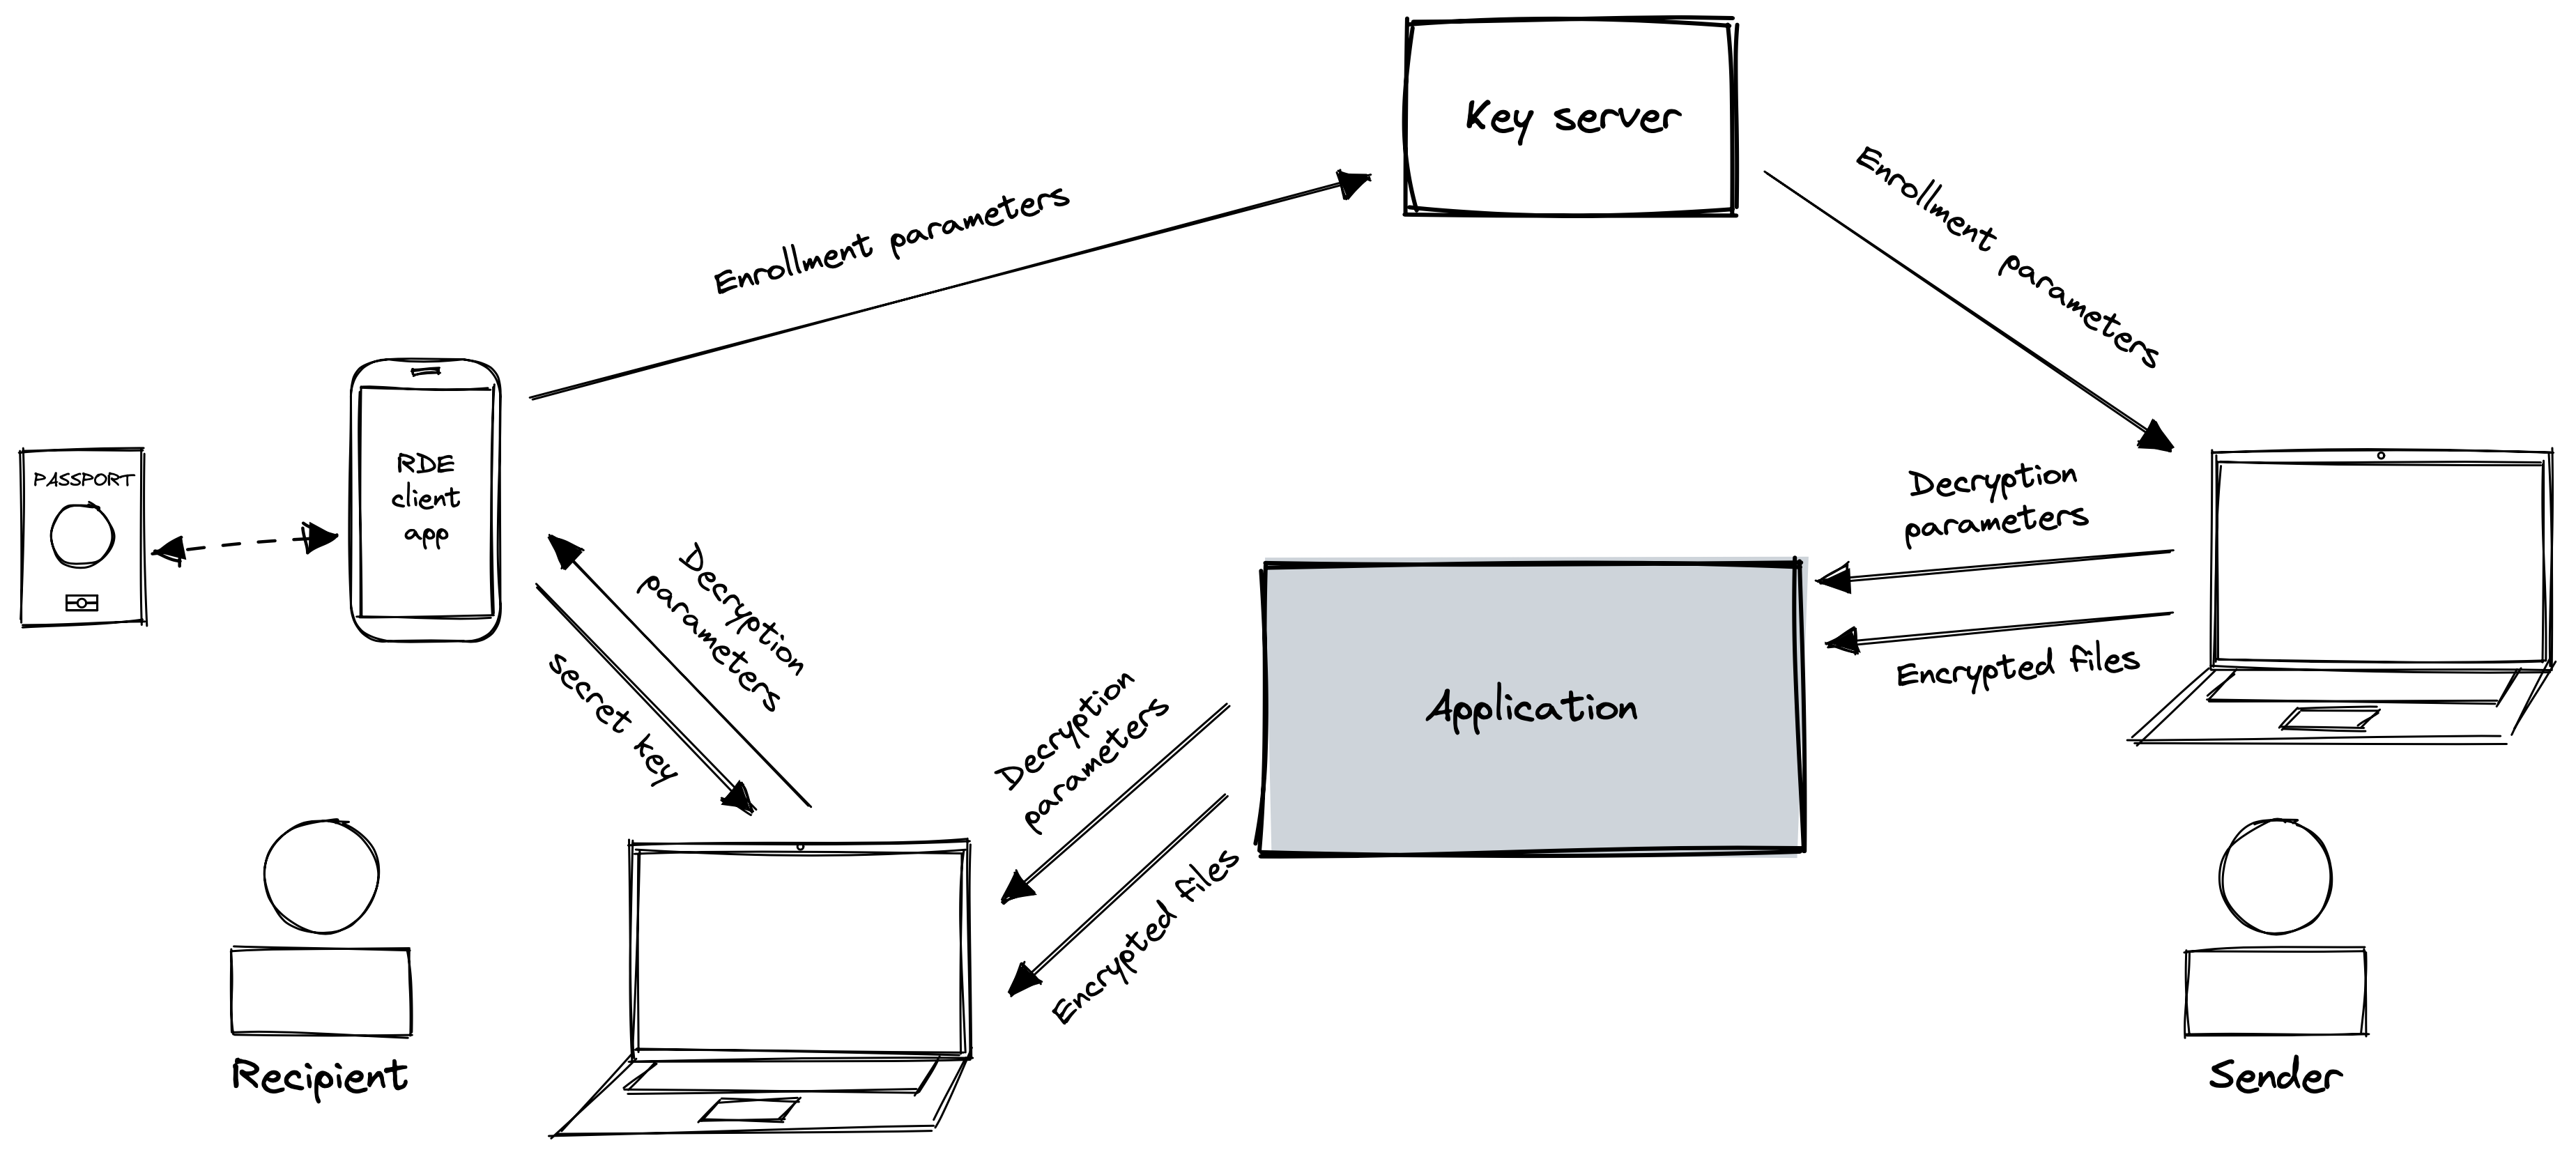
\includegraphics[width=\textwidth]{imgs/RDE infra overview}
    \caption{Overview of the RDE prototype infrastructure.
    A more detailed figure for each phase of RDE is included in Figure~\ref{fig:rde-detail}.}
    \label{fig:rde-prototype-infrastructure-overview}
\end{figure}

\begin{figure}
    \centering
    \begin{subfigure}[b]{0.5\textwidth}
        \centering
        
\includegraphics[width=\textwidth]{imgs/RDE enrollment detail}
        \caption{Enrollment}
        \label{fig:rde-enrollment-detail}
    \end{subfigure}\\
    \vspace{1cm}
    \begin{subfigure}[b]{0.8\textwidth}
        \centering
        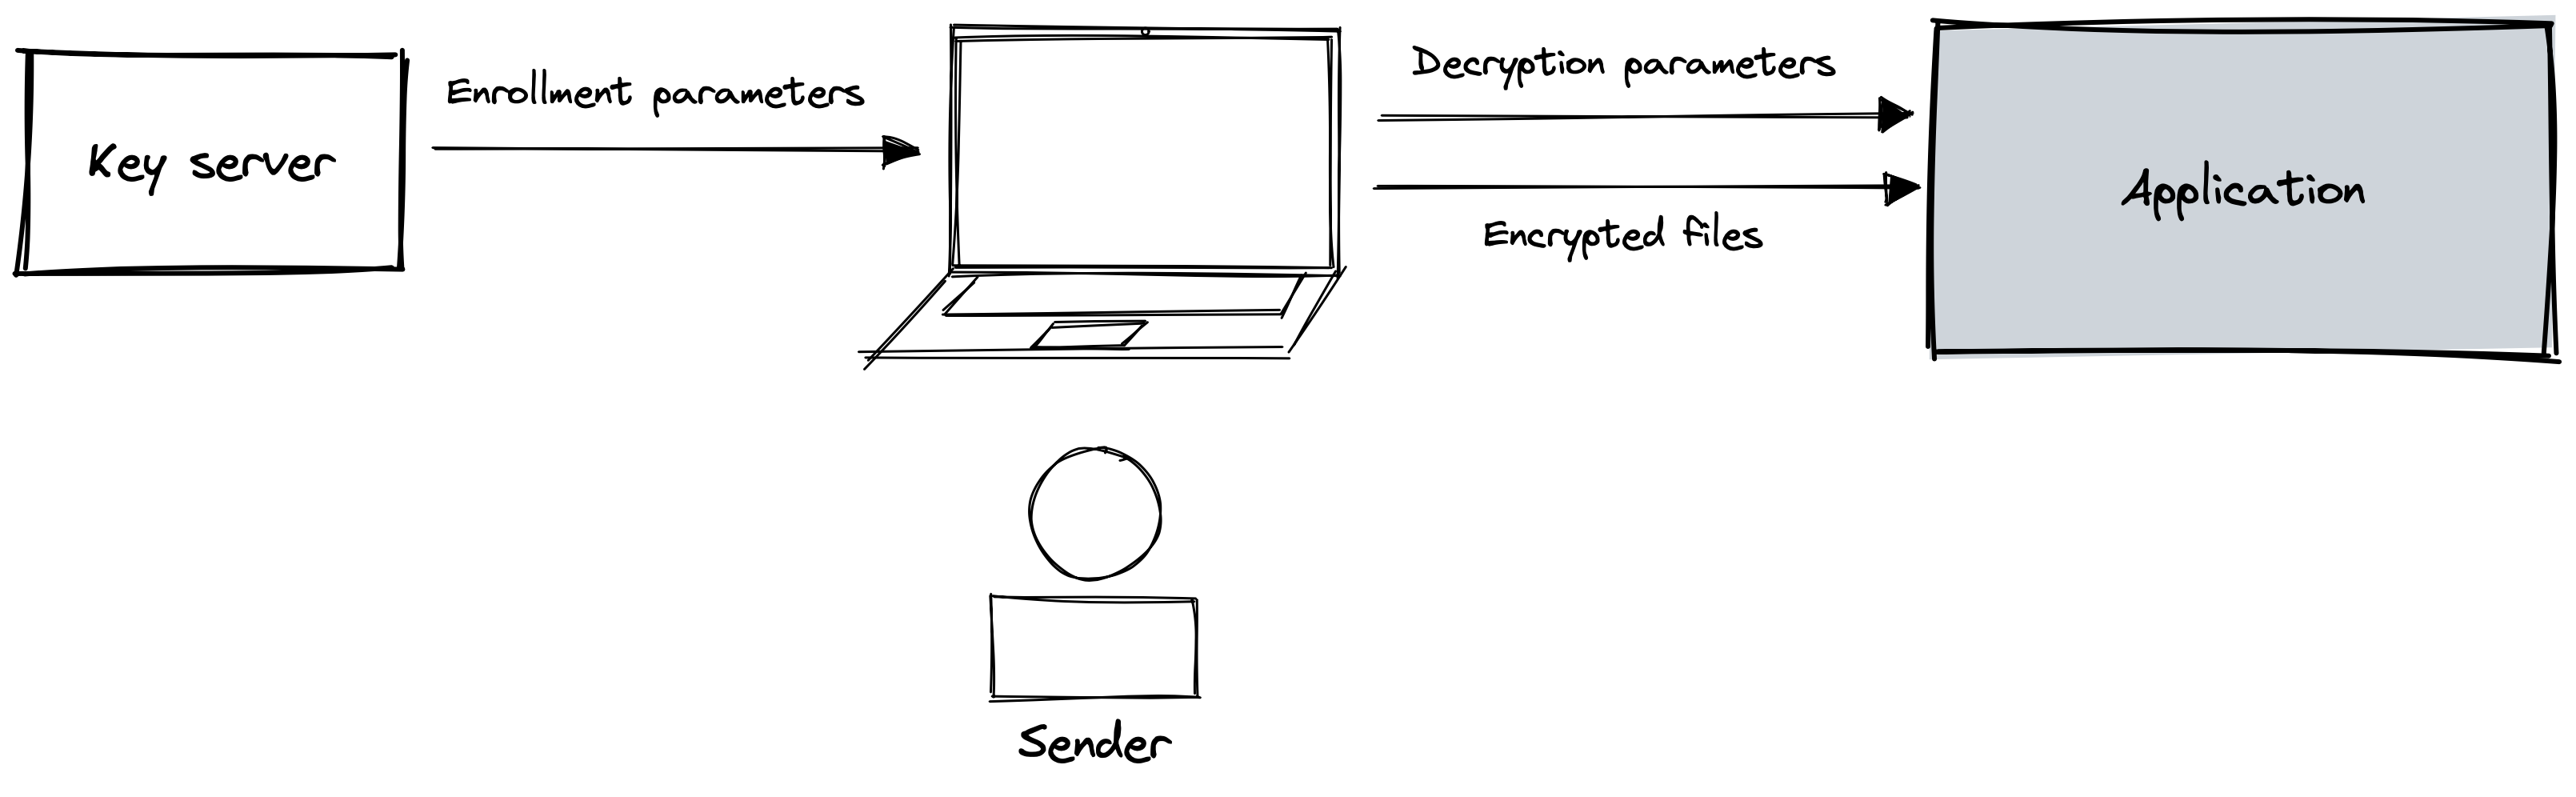
\includegraphics[width=\textwidth]{imgs/RDE keygen detail}
        \caption{Key generation}
        \label{fig:rde-keygen-detail}
    \end{subfigure}\\
    \vspace{1cm}
    \begin{subfigure}[b]{0.8\textwidth}
        \centering
        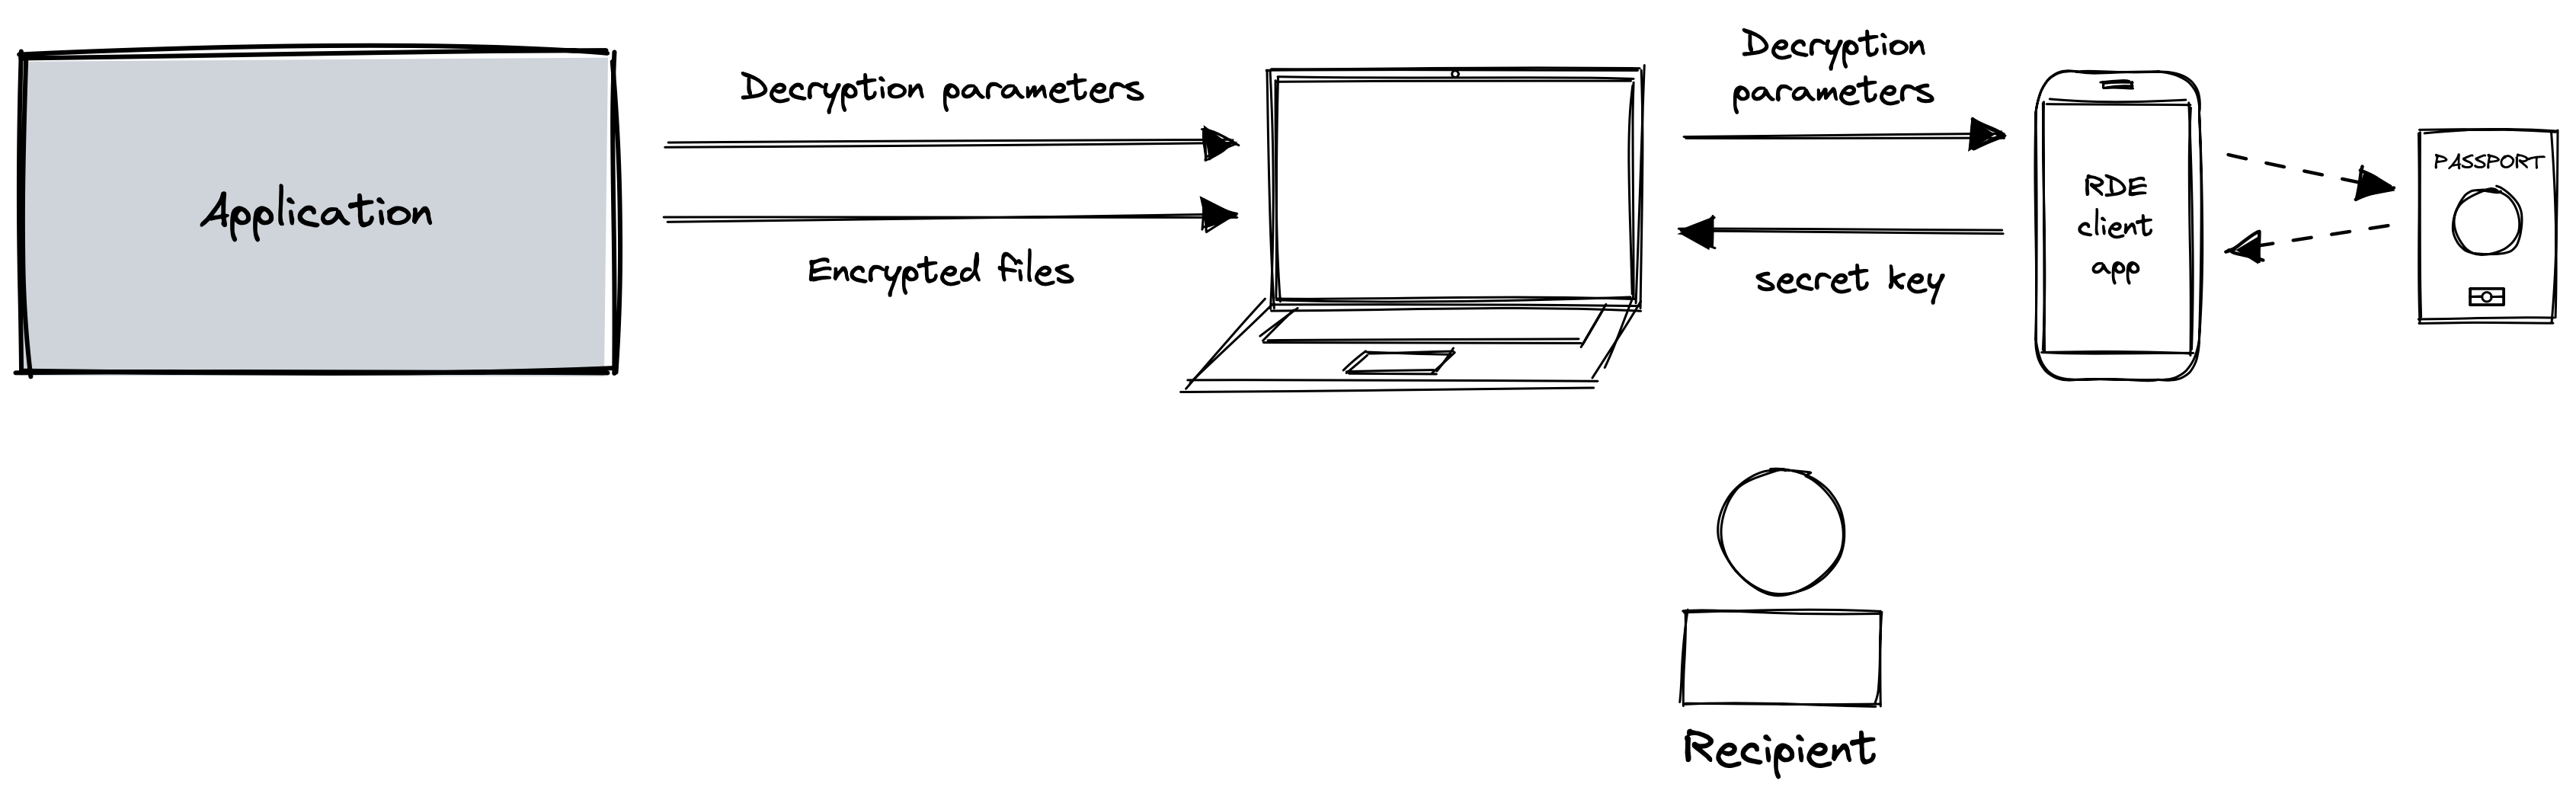
\includegraphics[width=\textwidth]{imgs/RDE decryption detail}
        \caption{Decryption}
        \label{fig:rde-decryption-detail}
    \end{subfigure}
    \caption{Interaction in the RDE prototype infrastructure in different phases.}
    \label{fig:rde-detail}
\end{figure}

\subsection{Notes on our implementation}\label{subsec:infrastructure-overview-notes-on-our-implementation}
For the prototype, we have implemented components that can be grouped into 3 categories:

First, there are the core RDE components that enable the enrollment, key generation and decryption (key retrieval) steps of the basic RDE scheme.
These consist of a Java library written in Kotlin for the interaction with the e-passport, and a TypeScript library for the key generation and passport emulation.
The latter is written in TypeScript, as it is intended to be used in a browser environment by the end user.
Their implementation is also independent of the actual application in FileSender, and can be used for other applications or infrastructures for RDE as well.

Second, there is a category of infrastructure components that are needed to make the RDE prototype work.
These are the RDE key server that stores enrollment data, the client app that enables enrollment en decryption and that uses the aforementioned library, and a simple proxy server that allows communication between the client app and the browser client of the recipient.
These components are minimal implementations that are sufficient for the prototype, but are not intended to be used in production in their current form, as they are not secure and do not have all the features that would be needed for a production system.
These components are still independent to the FileSender application, and can be used for other applications as well that use the same infrastructure.

Finally, there is the integration of RDE in the FileSender application itself.
Here, minimal changes have been made to the FileSender application to enable the RDE functionality.

\section{Core components}\label{sec:core-components}
The core components of the RDE prototype are the Java library (written in Kotlin) and JavaScript library (written in TypeScript) for key generation that provide the cryptographic functionality for the RDE scheme.
This includes the interaction with the e-passport for enrollment, the key generation and the decryption (key retrieval) steps.
The Java library basically forms a wrapper around the JMRTD library\footnote{\url{https://jmrtd.org}} for interaction with an e-passport and uses the BouncyCastle library\footnote{\url{https://www.bouncycastle.org}} for the cryptographic operations.
The JavaScript library is intended to be used in a browser environment by the end user and does not implement any steps that require interaction with the passport.
In the future, however, it could be interesting to implement this in the browser as well, as this would allow for a more seamless user experience.
This would require hardware support for NFC in the browser.

\subsection{Data classes}\label{subsec:data-classes}
There are several data classes that are used to store data / messages within the RDE protocol.
For our prototype, we have chosen for simple JSON objects, as they are easy to work with and can be easily converted to and from byte arrays.

\subsubsection{\textsf{RDEEnrollmentParameters}}\label{subsubsec:rdeenrollmentparameters}
The \textsf{RDEEnrollmentParameters} class is used to store the enrollment parameters for an e-passport.
This class includes the following fields:
\begin{itemize}
    \item \textsf{documentName}: a user-chosen name for the e-passport (mnemonic name), which is used to identify the e-passport towards the user (for example ``\textsf{My passport (******ABC)}'', showing the last 3 digits of the 9-digit document number).
    \item \textsf{rdeDGId}: the data group ID of the data group to read for RDE (usually 14).
    \item \textsf{rdeDGLength}: the number of bytes to read for RDE (usually 223, the maximum plaintext size for which the ciphertext fits in a single APDU).
    \item \textsf{rdeDGContent}: the plaintext contents of the data group to read for RDE (usually the first 223 bytes of the data group, or the full data group if we do include the EFsod in the enrollment parameters), as a hexadecimal string.
    \item \textsf{caOID}: the OID of the CA protocol supported by the e-passport.
    \item \textsf{piccPublicKey}: the public key of the CA protocol supported by the e-passport, as a hexadecimal string ASN.1 X9.62 TLV (Tag-Length-Value)-encoded public key (according to ICAO specification, X9.42 for RSA based DH and TR-03111 for ECDH~\cite{icao9303securitymechanisms}).
    \item \textsf{securityData}: the contents of EFsod, as a hexadecimal string, or null if the EFsod is not included in the enrollment parameters.
    \item \textsf{mrzData}: the contents of DG1, as a hexadecimal string, or null if the MRZ is not included in the enrollment parameters.
    \item \textsf{facialImageData}: the contents of DG2, as a hexadecimal string, or null if no facial image is included in the enrollment parameters.
\end{itemize}

\subsubsection{\textsf{RDEKey}}\label{subsubsec:rdekey}
The \textsf{RDEKey} class is used to store a generated RDE key, as generated by a sender.
It consists of the secret key (byte array) that can be used to encrypt an decrypt messages, and the decryption parameters that can be made public and that are used together with the e-passport to retrieve the secret key.

\subsubsection{\textsf{RDEDecryptionParameters}}\label{subsubsec:rde-decryption-parameters}
The \textsf{RDEDecryptionParameters} class is used to store the decryption parameters that are used to retrieve the secret key.
It consists of the ephemeral public key chosen by the sender and the protected command that should be sent to the e-passport to retrieve the secret key.
The public key is a X.509 hexadecimal encoded ASN.1 DER string according to ICAO specification (X9.42 for RSA-based DH and TR-03111 for ECDH~\cite{icao9303securitymechanisms}), and the protected command is encoded as a hexadecimal string.
Additionally, the OID\footnote{Object identifier, a globally standardized identifier for, among others, cipher suites.} of the CA algorithm is stored, as having this information saves us a step in the decryption process.

\subsection{Enrollment}\label{subsec:enrollment}
Enrollment is only included in the Java library, as it requires interaction with the e-passport.
During enrollment, first, the security info is read from the e-passport in order to determine if the e-passport supports PACE or if we should fallback to BAC for our first level of secure messaging.
If PACE is supported, we use PACE to authenticate to the e-passport, otherwise we use BAC.

After authentication, we read the data group that is chosen to be used for RDE.
Usually, you want this to be data group 14, as this group is usually of sufficient size and does not contain privacy sensitive data, but other data groups that can be read without Terminal Authentication are also supported.
If enrollment with MRZ data is chosen, we also read data group 1, which contains the MRZ data.
If enrollment with facial image data is chosen, we also read data group 2, which contains the facial image data.
Finally, we also read the EFsod, which contains the security data of the e-passport.

Then, we perform passive authentication with the information from the EFsod.
Note that in the current implementation, we do not check the certificate chain of the EFsod, as this is not necessary for the prototype and would require us to include a certificate store with trusted certificates.
In the future, this should be added to the implementation.

For enrollment, apart from the data group to use for RDE, users can also choose the number of bytes to read from that data group, $n$ or \textsf{rdeDGLength}.
This usually is 223, as this is the maximum plaintext size for which the ciphertext fits in a single APDU, but can also be less if the user agrees with weaker security.
Note that the data group must be large enough to actually read the number of bytes chosen by the user.
Especially data group 1 is too small to read 223 bytes, so we recommend using data group 14 for enrollment.

If enrollment with security data is chosen, we include the EFsod in the enrollment parameters, together with the full contents of the RDE data group.
If enrollment with MRZ data is chosen, we also include the MRZ data in the enrollment parameters, and similarly for facial image data.
If no security data is included, we only include the first $n$ bytes of the RDE data group, as this is the maximum plaintext size for which the ciphertext fits in a single APDU and we thus do not need more data.
If we do include security data, we must include the full RDE data group, as the hash of the RDE data group otherwise will not verify with the EFsod.

We also include the OID of the CA protocol supported by the document, as this is needed to determine the public key format, cipher algorithms and key length during key generation.

Finally, the enrollment parameters include a document name, which functions as a mnemonic name to identify the document towards the user (in case the user has multiple documents enrolled).

\subsection{Key generation}\label{subsec:key-generation}
Key generation is included in the JavaScript library, as it does not require interaction with the passport and is expected to run in the browser of a sender.
For completeness, however, we also include key generation in the Java (Kotlin) library, as it is useful for testing purposes and could potentially be useful for other applications when a server wants to encrypt messages for a user.
However, verification of the enrollment parameters is not yet implemented in the Java (Kotlin) library.
Only the TypeScript library currently implements verification of the enrollment parameters.

The key generation takes the enrollment parameters as input, and generates a secret key and decryption parameters.
This is done by first generating a ephemeral key pair for the offline CA (EC)DH key agreement, compatible with the CA protocol supported by the e-passport.
We then compute the shared secret using the ephemeral private key and the public key of the e-passport.
From the shared secret, we derive the KMAC and KENC keys according to the ICAO specification for the supported CA protocol.

The most significant step is then to emulate the e-passport response to a READ BINARY command for the RDE data group, using KENC to encrypt the data group and KMAC to compute the MAC.
This results in the emulated ciphertext, which is then used to generate the secret message key by simply taking the SHA-256 hash of the ciphertext.
We also generate the encrypted READ BINARY command with KENC and KMAC and store this, together with the ephemeral public key, in the decryption parameters.

The main difference between the key generation in the JavaScript (TypeScript) and Java (Kotlin) library is that the Java library uses the BouncyCastle library for all cryptographic operations and implementations from JMRTD, while for the JavaScript library these are not available.
The JavaScript library also cannot use the WebCrypto API for these steeps, as it does not support all algorithms and curves that are used in the ICAO specifications.
We therefore use custom crypto libraries for emulating the passport response and generating the protected command.
For more details, we refer to our source code.

\subsubsection{Verification of enrollment parameters}\label{subsubsec:verification-of-enrollment-parameters}
Before generating the secret key, we can verify the enrollment parameters to authenticate the document holder as described in Chapter~\ref{ch:rde-with-document-holder-authentication}.
This, naturally, is only possible if the enrollment parameters include security data.

First, the hashes on the chosen RDE data group, and optionally the MRZ data and facial image data, are verified against the hashes in the EFsod.
Then, the hash on the full EFsod is verified, followed by the signature on this data.
Finally, the certificate chain of the EF.SOD is verified against a trusted certificate store.

Any user can choose their own trusted certificates.
This means that a user can determine themselves which certificates from which issuing states they trust.
For the prototype, we use 13 certificates from the Dutch government Country Signing Certificate Authority (CSCA)\footnote{\url{https://www.npkd.nl}}.
Parsing a `Masterlist file' that contains a list of certificates from multiple CSCAs not yet implemented.
Certificates need to be provided individually in PEM format.
Also CRL's (Certificate Revocation Lists) are not yet implemented.

\subsection{Decryption (key retrieval)}\label{subsec:decryption-key-retrieval}
Decryption is only included in the Java library, as it requires interaction with the e-passport.
During decryption, similar to enrollment, first, the security data of the e-passport is read from the e-passport and either PACE or BAC is used to authenticate to the e-passport.
Then, we perform Chip Authentication with the ephemeral public key from the decryption parameters.
The e-passport will now further communicate with the reader using the shared secret with the sender who created the decryption parameters.
We then send the protected command from the decryption parameters to the e-passport, which results in ciphertext contents of the RDE data group.

We derive the secret message key from the ciphertext by simply taking the SHA-256 hash of the ciphertext.

We reiterate that the ciphertext that forms the basis for the secret key, is sent in the clear from the e-passport to the reader (that computes the SHA-256 hash).

\subsection{Cryptography implementations}\label{subsec:cryptography-implementations}
As mentioned earlier, cryptographic operations in the Kotlin library use JMRTD and BouncyCastle.
This is the obvious choice, as JMRTD is a solid library that implements communication with e-passports, and already uses BouncyCastle.

For the JavaScript libraries, the preferred solution would be to use the WebCrypto API, as it is the most secure and most efficient implementation.
The WebCrypto API, however, does not support all cryptographic operations that are required for emulating a passport, such as AES-CMAC or elliptic curve cryptography with brainpool curves.
That is why we have chose to use the following cryptographic libraries for emulating e-passport commands and responses:

\begin{itemize}
    \item \textsf{@peculiar/x509}
    \item \textsf{indutny/elliptic} (for ECC on arbitrary curves)
    \item \textsf{indutny/hash.js}
    \item \textsf{rosek86/aes-cmac} (for AES-CMAC)
    \item \textsf{leonardodino/aes-ts} (for AES-CBC and AES-ECB with no padding)
\end{itemize}

\section{Infrastructure components}\label{sec:infrastructure-components}
The infrastructure components of the RDE prototype are the key server, the proxy server and the reader app.
They function as a minimal implementation of the RDE prototype and work independently of the FileSender application (or any other application for that matter).

\subsection{Key server}\label{subsec:key-server}
The key server in its most simple form is a simple REST API that stores the enrollment data and allows users to query it.
Our implementation is written in Python and uses the Django web framework.
Users can register and log in to the key server using SURFconext, which is a federated identity provider.
Via SURFconext, the key server receives the user's email address which will be used to link the enrollment data to.
Users can then use the reader app to enroll their e-passport and push the enrollment data to the key server.

\subsubsection{Querying the key server}\label{subsubsec:querying-the-key-server}
The key server provides a REST API for querying the enrollment data based on the user's email address.
The key server will then return the enrollment data for the user, if it exists.

It is important to note that by storing all enrollment data on the key server, this key server contains a lot of privacy sensitive information.
If users choose to use document holder authentication during enrollment, the key server might contain the MRZ data and facial image data of the user.
We should thus be careful with making the key server available to the public.
Probably, we should only allow certain authenticated users to query the key server.
This is not implemented in the prototype and is topic for further discussion.

\subsubsection{Key server security}\label{subsubsec:key-server-security}
There are a number of security assumptions that we make about the key server.
\begin{itemize}
    \item For senders, we do trust the key server to return the correct enrollment data for a user's email address.
    \item For senders, we do \emph{not} need trust the key server to not modify the enrollment data if the data includes document holder authentication.
    Senders can verify the enrollment data themselves.
    \item For recipients enrolling at the key server, we do trust the key server to handle the enrollment data securely with respect to the user's privacy.
\end{itemize}
In this sense, the security assumptions towards the RDE key server are similar to those of other key servers, such as for PGP.

\subsubsection{Notes on our implementation}\label{subsubsec:keyserver-notes-on-our-implementation}
The implementation of the key server for our prototype is very minimal.
The API for querying the key server is very simple and does not include any authentication for querying users or rate limiting.
The key server also does not verify the enrollment data upon receiving it.
Finally, it provides no way to delete enrollment data.
The process of scanning a QR code for enrolling e-passports is an easy implementation, but not very user friendly and not very secure.
For a production system, these features should be implemented.

\subsubsection{SURFconext and eduID}\label{subsubsec:surfconext-and-eduid}
One approach for implementing a production key server at SURF is to integrate it within eduID, another service SURF offers.
eduID can be considered as an universal identity service that contains different attributes about a user.
In contrast to regular SURFconext, where attributes are provided by institutions, eduID attributes are stored by SURF itself.
This means that eduID can be used to store attributes that are not provided by institutions, such as the RDE enrollment parameters.

A user's RDE `public key' (enrollment parameters) could thus be stored as attributes in eduID.
This would, however, still require a key server to be implemented for querying the enrollment parameters for users.
It is thus questionable whether this would be a good approach for implementing an RDE public key server at SURF, at least not necessarily for filesender applications, where senders need to query for enrollment parameters of other users.
Only in situations where the sender is a server, encrypting information for the user itself, would this approach be useful.

\subsection{Proxy server}\label{subsec:proxy-server}
In order to achieve true end-to-end encryption, the browser and the app need to be able to communicate with each other.
This is not easily possible, as we cannot assume that the browser and the app are on the same network (even if they are, they can probably not communicate directly).
Therefore, we have created a proxy server that acts as a middleman between the browser and the app.
The sole purpose of this server is to relay messages between the browser and the app.
It is not involved in the actual encryption process, nor should it have any security critical role.
The proxy server is implemented in Python and uses the Flask web framework.
The proxy server simply allows websockets to be opened between the browser and the app and relays messages between them.

\subsubsection{Decryption handshake protocol} \label{subsubsec:decryption-handshake-protocol}
In order to facilitate end-to-end encryption between the browser and the app, we have created a simple protocol for the decryption handshake.
The protocol is very simple and consists of the following steps:
\begin{enumerate}
    \item The browser opens a websocket connection to the proxy server on a unique URL.
    \item The browser presents a QR code to the user that contains the URL of the websocket connection.
    \item The user scans the QR code with the app.
    \item The app opens a websocket connection to the proxy server on the same URL.
    \item The app generates a ephemeral key pair and sends the public key to the browser.
    \item The browser generates a ephemeral key pair and a random IV and sends those back to the app.
    \item Both parties perform a Diffie-Hellman key exchange using the ephemeral key pairs.
    Both parties now have the same shared secret and can communicate with each other using this shared secret.
    \item The browser sends the decryption parameters to the app, encrypted with the shared secret and the IV.
    \item The app decrypts the decryption parameters and uses them to retrieve the secret key from the passport.
    \item The app sends the retrieved secret message key to the browser, encrypted with the shared secret and the IV.
\end{enumerate}

We use ECDH with the NIST P-384 curve for the Diffie-Hellman key exchange.
For further communication, we use AES-256-CBC with a 128-bit IV.
Keys are encoded as JWKs.

We expect the connections with the proxy server to use TLS (WebSocket Secure) (and strongly rely on this for security).
This means that the proxy server will not be able to read the messages sent between the browser and the app.

This protocol is implemented in a TypeScript library for decryption, and in the reader app.
Because this protocol, however, is not part of the RDE scheme itself, we do not discuss it in depth.

\subsubsection{Attacks on the proxy server}
The proxy server is a potential point of failure in our prototype infrastructure.
An active MITM attacker could intercept the ECDH key exchange and this way be able to read the secret key that is transferred from the reader app to the browser.
This can easily be achieved by authenticating the shared secret between the browser and the app by showing a message to the user that they need to confirm on both devices, or by letting the app create a simple linking code that the user needs to enter on the browser before proceeding.
For the implementation in our prototype, we have chosen to not implement such security measures, as this does not relate to the actual RDE protocol and we consider it out of scope for this prototype.
For production systems, however, we should definitely consider implementing security measures against MITM attacks.

Phishing attacks are also a potential threat, as the user might be tricked into scanning a QR code that is not generated by the browser.
This also results in the user's secret key being leaked to the attacker.
This can be solved, too, by showing a message to the user that they need to confirm on both devices.
We have not implemented this in our prototype either, as it is not part of the RDE protocol.

\subsubsection{Notes on our implementation}
The implementation of the proxy server for our prototype is very minimal.
It does not implement any authentication or rate limiting, nor does the proxy server verify the messages sent between the browser and the app actually follow the decryption handshake protocol.
For a production system, these features should be implemented, as well as security measures against MITM attacks.

\subsection{Reader app}\label{subsec:reader-app}
The reader app is a simple Android app that uses the Java (Kotlin) library to read the e-passport.
It can be installed on a mobile device and is used to read the e-passport and retrieve the decryption key.

The reader app does not store any data itself.
There is thus no reason for the reader app to be installed on the user's personal device.
Any device that can interact with the e-passport can be used.

At decryption, however, the reader app will receive the secret key and thus must be trusted with this key.
Additionally, the ciphertext that the secret key is formed from, is sent in the clear from the e-passport to the reader app.
This means that we do have strong trust requirements for the reader app, the device it is installed on, and the environment in which it is used.

At enrollment, we do not have such strong trust requirements.

\subsubsection{Notes on our implementation}
The implementation of the reader app for our prototype is very minimal.
Especially, the user interface is very basic and does not provide any feedback to the user.
For a production system, this should be improved, not only for the user experience, but also to prevent phishing attacks.

\section{FileSender integration}\label{sec:filesender-integration}
The RDE implementation in the Filesender application is a simple extension of the existing application.
We have tried to keep the changes to the application as minimal as possible, while still allowing for the RDE functionality to be implemented.

It is important to note that we do not implement the filesender encryption scheme from~\cite{verheul2020secure}.
In his paper, in section 4, Verheul describes its own encryption scheme to encrypt the actual files that are sent.
The filesender project, however, already has its own file encryption scheme based on PBKDF2 and AES-256.
Therefore, we have chosen to use this existing encryption scheme, and only implement the RDE key agreement steps on top of it.
This means that the secret key that results from RDE, is used as input for a PBKDF2 key derivation function, which is then used to encrypt the files that are sent.

An overview of the RDE infrastructure integrated in the FileSender application is shown in Figure~\ref{fig:filesender-infrastructure}.
\begin{figure}
    \centering
    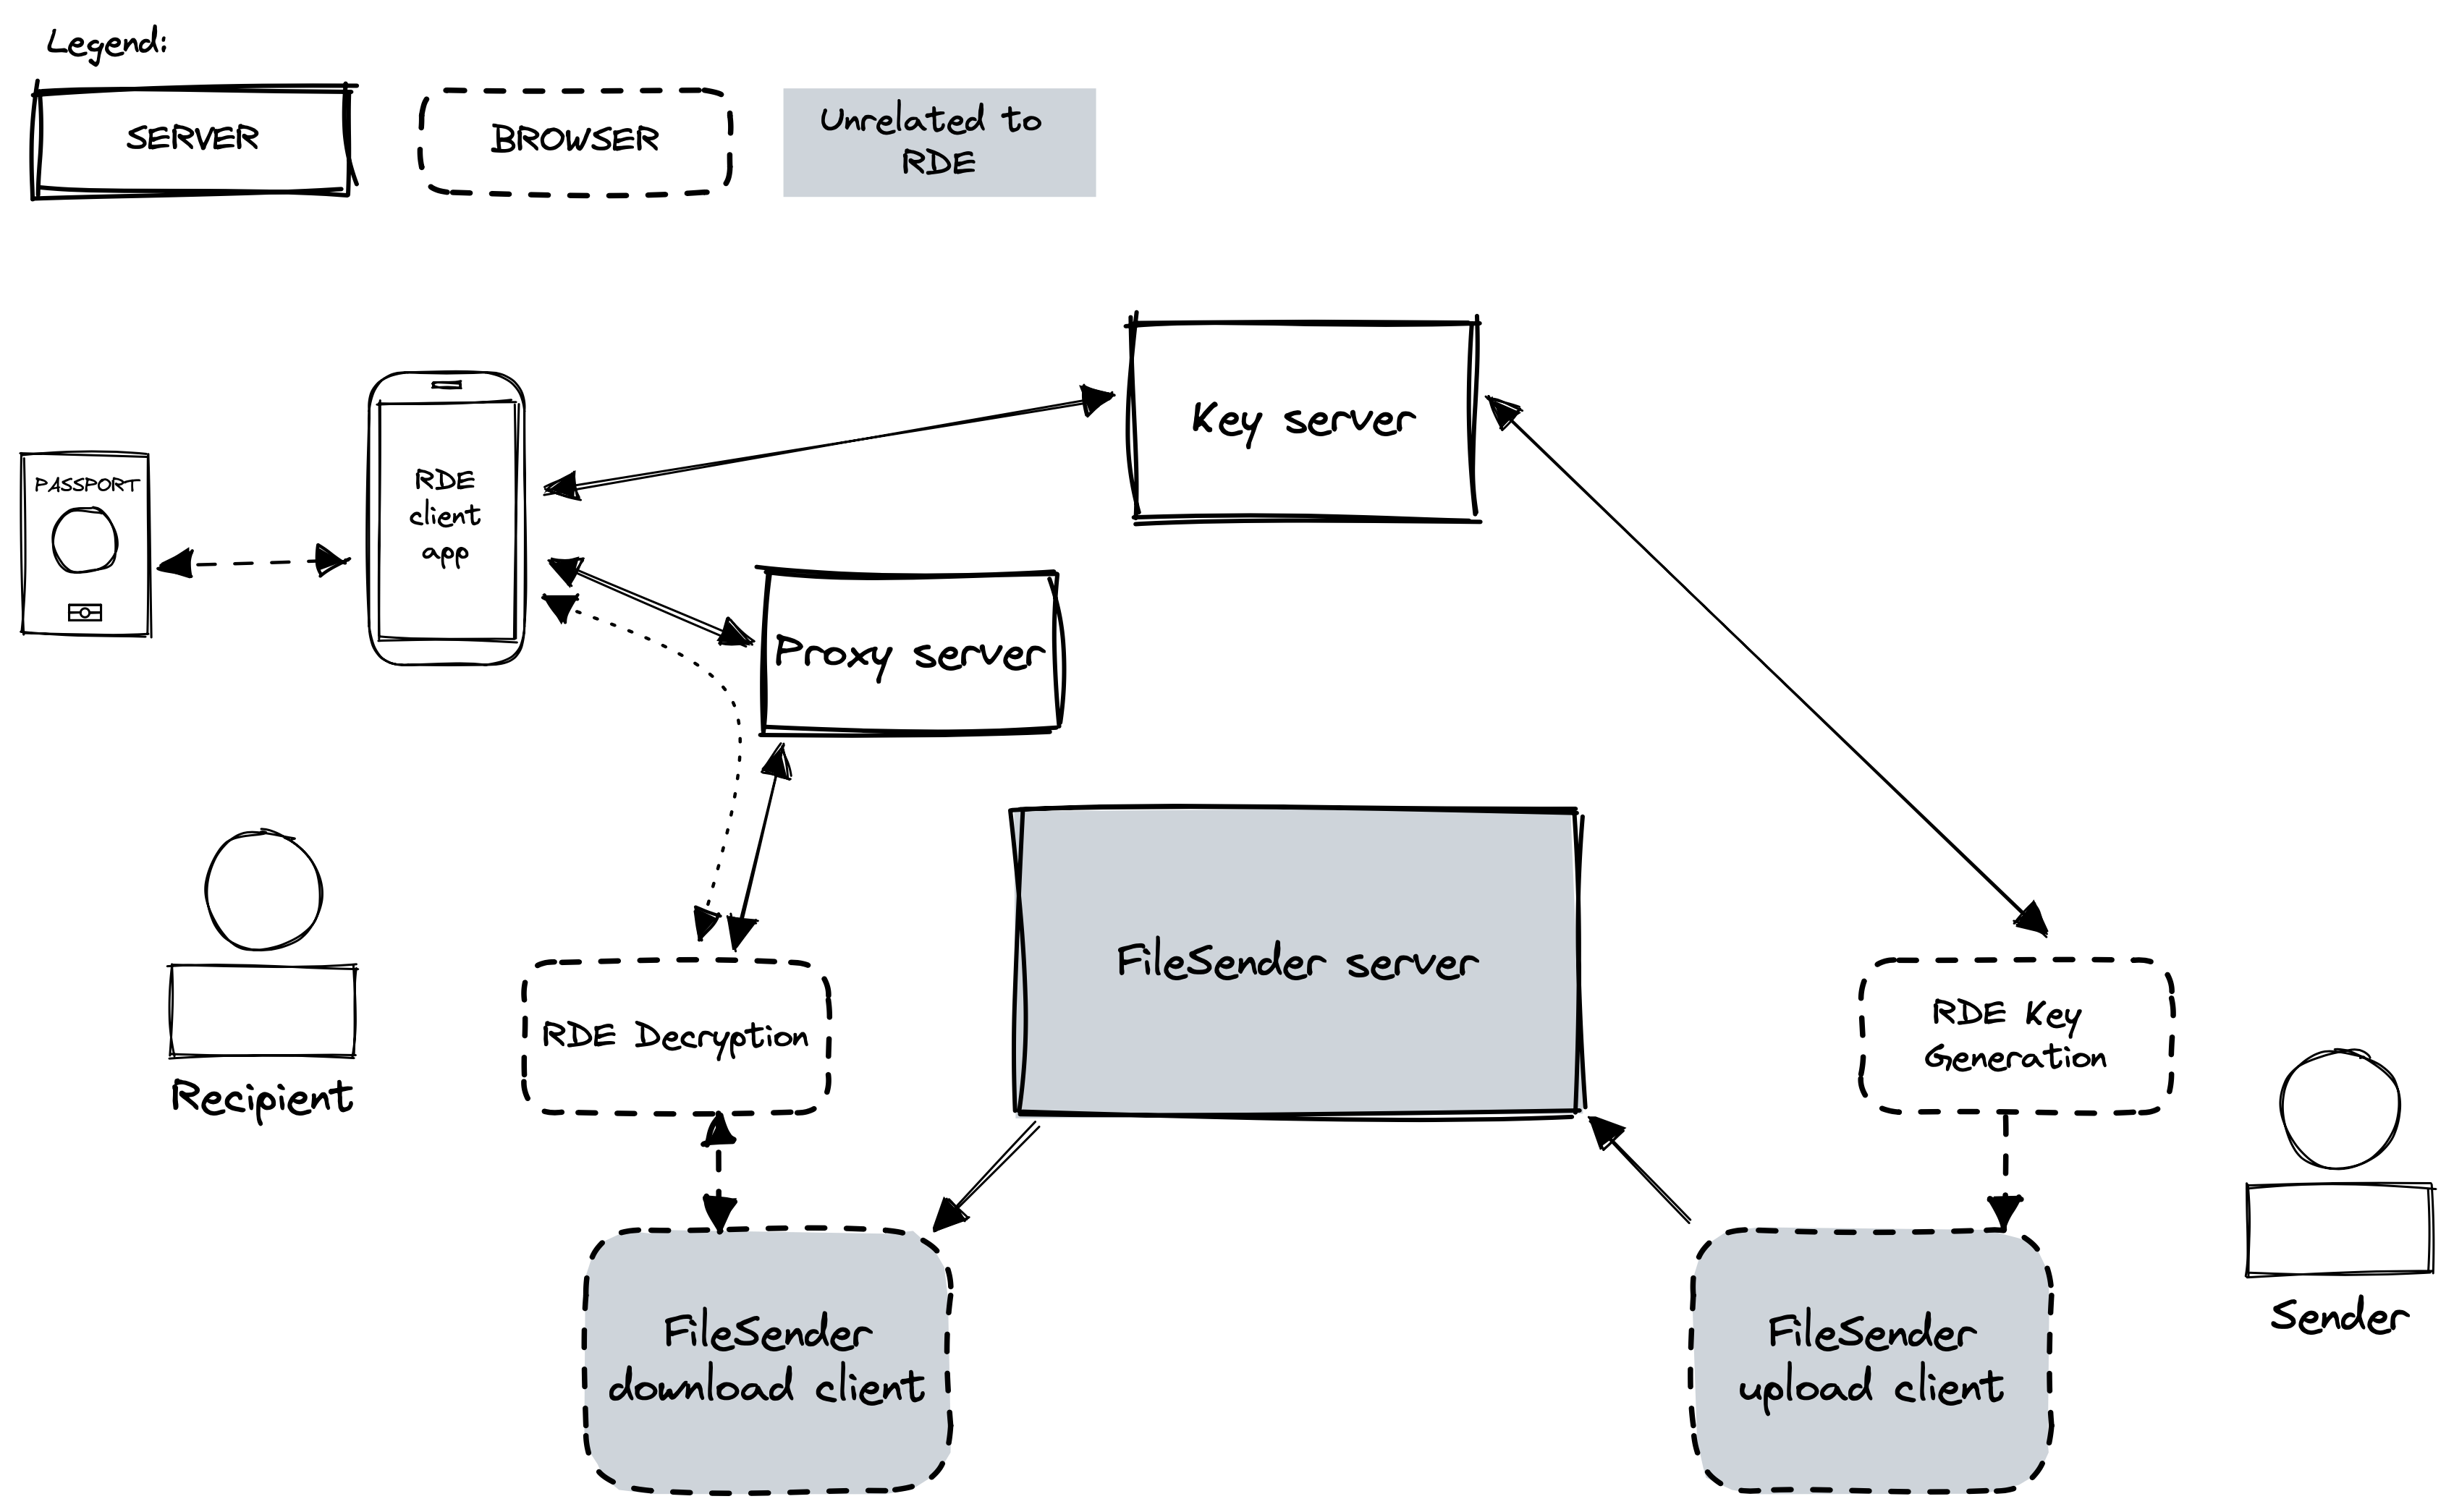
\includegraphics[width=\linewidth]{imgs/Filesender infra overview}
    \caption{Overview of the RDE infrastructure integrated in the FileSender application.}
    \label{fig:filesender-infrastructure}
\end{figure}

\subsection{File upload}\label{subsec:file-upload}
Upon uploading a file, the user is presented with the possibility to choose between the regular FileSender encryption scheme and the RDE encryption scheme.
If the user chooses the RDE encryption scheme, the user is presented with a field to query a key server with a certain email address.
The browser queries the key server for the provided email address and retrieves the enrollment parameters.
The user is then presented this list with enrollment parameters that they can choose from.

\subsubsection{Verification of the enrollment parameters}
After the user has chosen an enrollment parameter, the browser verifies the enrollment parameters.
When the enrollment parameters do not pass the verification, the user is presented with an error message.
Otherwise, a notification is shown to the user with the validated information.
There are several possibilities:

\begin{itemize}
    \item The enrollment parameters could not be verified, because no security data was included.
    The user can still proceed, but the document holder is not authenticated in any form.
    We thus fully rely on the key server for the identity of the document holder.
    \item The enrollment parameters have been verified to be from a valid e-passport.
    The issuing country and validity of the signature are shown to the user.
    \item The enrollment parameters have been verified to be from a valid e-passport and the document holder's MRZ data is included.
    In this case, additionally, the MRZ data is shown to the user.]
    \item Additionally, the facial image of the document holder is shown to the user.
\end{itemize}

In a production system, we probably want to verify the enrollment parameters before they are shown to the user for selection.
The FileSender application could also put extra restrictions on what enrollment parameters are allowed to be used.
Wwe could only accept verified enrollment parameters, enrollment parameters with MRZ data, or only accept enrollment parameters that are valid for a certain period of time.
For example, it might be desirable to disallow senders to select enrollment parameters that expire before the end of the file transfer availability period, as to prevent the document holder from being unable to decrypt the file.
These are all topics for further consideration.

\subsubsection{File encryption}
After the user has chosen the RDE document to encrypt for and verified the enrollment parameters, the browser generates an RDE key.
The decryption parameters are send to the FileSender server and stored in its database.
The secret key is used as the password for the PBKDF2 key derivation function that is already implemented in the FileSender application (for password-based encryption).

We note that the reason for choosing to use PBKDF2 here is only for the convenience of developing this prototype.
In fact, there is no reason to use PBKDF2 here, as the RDE secret key is already a random key.

\subsection{File download}\label{subsec:file-download}
When the recipient tries to download a file that is encrypted with RDE, they are presented with a popup that asks them to scan a QR code with their reader app.
This triggers the RDE decryption handshake protocol as described in Section~\ref{subsubsec:decryption-handshake-protocol}.
This results in the retrieval of the secret key, which was used to encrypt the files.
This key is then again used in the PBKDF2 key derivation function to finally decrypt the files.

Note that we only find out if the decryption was successful after the first blob of a file was decrypted.
If a user would try decryption with the wrong document, the key retrieval steps would not necessarily fail, but result in a different secret key and thus only the decryption would fail.
We will, however, only find out after the first blob of a file was decrypted.
This is also the current behavior of the FileSender application for password-based file encryption.

\subsection{Notes on our implementation}\label{subsec:notes-on-our-implementation}
The implementation of the RDE integration in the FileSender application for our prototype is very minimal.
The current FileSender code base, especially with regards to the UI and browser encryption and decryption, is not very modular.
This makes it difficult to integrate RDE in a clean way.
We know that the FileSender developers are working on a new version of the application, which will feature a new UI and hopefully a more modular code base.
We expect that the integration of RDE in the new version of the FileSender application will be much easier and cleaner given the modularity of the RDE components that we developed.

\subsubsection{FileSender CLI}
We also note that the FileSender application provides a CLI tool.
We have not implemented RDE for this CLI tool, as this has not been a priority for us.

\subsubsection{The recipient}
The current FileSender integration does not enforce that the download link of the transfer is only shared with the email address that is associated with the enrollment parameters.
For a production system, this probably should be enforced for usability reasons.

\subsubsection{User interface}
In line with the rest of our prototype, the user interface of the RDE integration in the FileSender application should be improved so users better understand what is going on and users do not make unfair assumptions about the security of the system.


    \chapter{Going forward}
\label{ch:going-forward}
In this chapter, we will discuss the next steps that need to be taken to bring the current prototype to a production-ready state, partially in addition to remarks that were made in the previous chapters.

\section{Key server}
\label{sec:key-server}
Most notably, a production-ready RDE key server needs to be developed, and possibly integrated into existing applications.
The whole enrollment process needs to be reworked to be more user-friendly and more secure.
We refer to the previous chapter for more details on this.

\section{User interface and user experience}
\label{sec:user-interface-and-user-experience}
The current prototype is a proof-of-concept, and thus, the user interface is not very user-friendly.
Errors are not handled very well, and the user is not informed about what is going on.
This needs to be improved.

Specifically the term `Remote Document Encryption' is not very user-friendly, and should be replaced with something more descriptive, such as `Passport/ID-based encryption'.
Terms like `security data', `MRZ data` and `facial image' should be replaced with better terms.
Regarding the MRZ data specifically, those terms should make clear to users the privacy implications of sharing this data.
Users should know that this data contains their full name, nationality, sex, date of birth, and document number, and understand the implications of publishing this data.
On the other hand, they should also understand that reading this data does not make it possible to commit identity theft.

\section{OCR in the reader application}
\label{sec:ocr-in-the-reader-application}
In order for the reader app to communicate with the e-passport, it needs to know the BAC key of the document (or the CAN, if the document has a CAN).
This BAC key is based on the document number, date of birth and expiry date of the document.
Currently, the reader application asks the user to enter this data manually.
This is not very user-friendly.
Instead, the reader application should be able to read this data from the printed MRZ on the document.
This can be done using optical character recognition (OCR).
For privacy reasons, this OCR should be done locally on the user's device, and not on a remote server, as the MRZ data could contain the personal number of the document holder (that SURF is not allowed to process).

\section{iOS support}
\label{sec:ios-support}
For the prototype, we have only developed a reader application for Android.
However, the same reader application should also be developed for iOS.
This is not trivial, as a powerful library like JMRTD is not available for iOS (in face, iOS just recently gave developers low level access to the NFC chip).
The \textsf{AndyQ/NFCPassportReader}\footnote{\url{https://github.com/AndyQ/NFCPassportReader}} library is available for iOS and seems to implement all the functionality that we need.

\section{Support for more document types (drivers licenses)}
\label{sec:support-for-more-document-types}
Currently, the prototype only supports e-passports and e-ID cards.
In The Netherlands, however, there are also e-driver's licenses, and e-residence permits.
It is almost certain that these documents can be used for RDE as well (with minimal changes to the reader app), but this has not yet been implemented.

\section{Encrypting for multiple keys}
\label{sec:encrypting-for-multiple-keys}
The current implementation allows senders to choose to encrypt a transfer for a single e-passport.
There might, however, be applications where it is useful to encrypt for multiple e-passports.
For example, if a transfer should be available to multiple people, but perhaps more importantly, if one person should be able to decrypt a transfer with either one of his documents (passport, identity card, driver's license).
This could greatly improve usability.
In order to achieve this, the integration of RDE within the encryption scheme of FileSender should be changed.
Instead of using the secret key from RDE directly for encrypting the files (after PBKDF2), files instead should be encrypted with a different key, and the RDE secret key should in its turn encrypt this key.
This way, multiple RDE keys can be generated, all to encrypt the file encryption key, so that multiple documents can ultimately decrypt the same transferred files.

When such changes are made to the FileSender integration, it would also be beneficial to not use PBKDF2 at all for RDE, as it is not required and does not truly offer additional security.

\section{Support for more ciphers}
\label{sec:support-for-more-ciphers}
Currently, the response emulation in RDE key generation step only supports ECDH for Chip Authentication key agreement with AES based ciphers after the key agreement.
This covers by far the most commonly used passports.
According to the ICAO specifications, however, there are also passports that use RSA-based DH for key agreement, and DES based ciphers after the key agreement~\cite{icao9303securitymechanisms}.
A first step would thus be to investigate what countries actually use these passports, and then decide whether those should be supported or not.
One could also argue that these passports are not very secure, and thus, we should not support them at all.

    \chapter{Further research}
\label{ch:further-research}
In this chapter, we will discuss the further research that can be done on the topic of application of Remote Document Encryption.
These are more fundamental research questions, in contrast to the more implementation-related topics that were discussed in the previous chapter.

\section{Split-key architecture}
\label{sec:split-key-architecture}
Currently, the decryption (key retrieval) step in RDE is based fully on the e-passport.
The secret key is retrieved fully from the e-passport.
This has some consequences.
In case a user loses his e-passport, however, there is no way for them to revoke their passport.
They surely could indicate at a key server that their passport is lost (after authenticating with their email, for example), hopefully preventing others from still using the passport's enrollment parameters to encrypt for.
Already encrypted documents that are already out there, however, cannot be revoked.

A possible solution to this problem is to use a split-key architecture.
In such an architecture, the secret key would not only be based on the response of the e-passport, but also on a secret key that is stored on a key server.
For decryption, the key server would thus also need to be involved.
To revoke a document, the user would simply need to revoke the key on the key server, making any future decryption attempts fail.

With such an infrastructure, also a PIN could be introduced that needs to be provided in order to unlock the key server's secret key part.
Introduction of a PIN would give us even more security, as it prevents stolen or lost passports from being used to retrieve the secret message key.
Note that this still does not bind the e-passport to a specific reader app.
The reader app itself still does not need to store any secret data itself.

\section{Biometric authentication}
\label{sec:biometric-authentication}
A PIN would be a nice addition to the RDE scheme, but it is not the only way to improve the security of the scheme.
A PIN can still leak or be shared with others.
An interesting alternative is to use biometric authentication.

Currently, SURF's eduID project is working on a system that authenticates users with their passport and biometric data.
This is based on a product from the company Verifai\footnote{\url{https://www.verifai.com}}.
Verifai offers a so-called \emph{liveness check}\footnote{\url{https://docs.verifai.com/sdk/android/components/liveness-check}} to verify the user is indeed the document holder and is actually present.
This is done by asking the user to blink, move their head, speak some words, and verifying this against the facial image in the passport.

It could be interesting to use this liveness check to authenticate the document holder both at enrollment, but more importantly, at decryption.
Only after the liveness check is performed, the key server, implementing a split-key architecture, should release its secret key part.
A drawback of this approach, however, is that the Verifai liveness check is performed in-app, and thus requires a certified reader app (we need to trust the app to perform the liveness check correctly).
This is a big change from the current prototype, where the reader app is not certified.

\section{Other readers}
\label{sec:other-readers}
Currently, the prototype uses an Android app as reader for e-passports (and an iOS app is still to be developed).
This is chosen as NFC-capable phones are commonly available at this moment.
However, there is no reason why reading e-passports should be limited to phones.
For example, a simple USB smart card reader could be used to read e-passports as well.

It would be interesting to investigate if it is possible to interface with a USB smart card reader from a web browser, and if so, how this could be used to read e-passports.
This way, using a reader app would not be required anymore.
This would also further simplify the infrastructure, because no proxy server and decryption handshake between browser and reader app would be required anymore.





    \addcontentsline{toc}{chapter}{Acknowledgements}
\chapter*{Acknowledgements}
I would like to thank Stephen Kellaway\footnote{\url{https://github.com/playtime222}} in particular, who has been working on a similar project for the Dutch RDW\footnote{\url{https://www.rdw.nl}} and who helped me a lot during the early stages of my project, getting the first version of my Kotlin library to work.

Apart from that, I would like to thank my supervisors at SURF, William van Santen and Nils Vogels, for being great conversation partners to discuss this project with. 


    \bibliographystyle{plain}
    \addcontentsline{toc}{chapter}{References}
    \renewcommand{\bibname}{References}
    \bibliography{references}

    \appendix
    \chapter{Glossary}\label{ch:glossary}
\paragraph{3DES} Triple DES (Data Encryption Standard). \textit{A symmetric key encryption algorithm (that is considered to be broken).}
\paragraph{AES} Advanced Encryption Standard. \textit{A symmetric key encryption algorithm.}
\paragraph{BAC} Basic Access Control. \textit{A protocol for authentication and key establishment using symmetric crypto challenge response (3DES), based on a key derived from the MRZ (document number, date of birth and date of expiry). Required to communicate with the an e-passport.}
\paragraph{CA (1)} Certificate Authority. \textit{A trusted third party that issues certificates.}
\paragraph{CA (2)} Chip Authentication. \textit{Authentication protocol of an eMRTD's for authenticating possession of the CA private key of a chip and for setting up stronger keys for further communication.}
\paragraph{CAN} Chip Authentication Number. \textit{A number that is used to authenticate a terminal towards an e-passport. It is a simple number printed om a card (like a password).}
\paragraph{CRL} Certificate Revocation List. \textit{A list of revoked certificates.}
\paragraph{CSCA} Country Signing Certificate Authority. \textit{The organization that is responsible for a country’s PKI.}
\paragraph{DG1} Data Group 1. \textit{A data group of an eMRTD that contains the personal data of the document holder.}
\paragraph{DG2} Data Group 2. \textit{A data group of an eMRTD that contains the facial image of the document holder.}
\paragraph{DG14} Data Group 2. \textit{A data group of an eMRTD that contains the Chip Authentication public key.}
\paragraph{DH} Diffie-Hellman. \textit{A key agreement protocol.}
\paragraph{DSC} Document Signer Certificate. \textit{A certificate on the EMRTD from the document signer.}
\paragraph{DS} Document Signer. \textit{The party that signs documents. The DS certificate is signed by the CSCA.}
\paragraph{ECDH} Elliptic Curve Diffie-Hellman. \textit{A key agreement protocol based on elliptic curve cryptography.}
\paragraph{EFsod} Document Security Document. \textit{A file on an eMRTD that contains hashes on all data groups, and a signature and public key from the Document Signer.}
\paragraph{E-passport} Electronic Passport. \textit{See eMRTD.}
\paragraph{eID} Electronic Identity Document. \textit{See eMRTD.}
\paragraph{eMRTD} Electronic Machine Readable Travel Document. \textit{See MRTD. A machine-readable travel document that contains an integrated circuit chip (IC) for contactless communication. Recognizable by a specific ICAO logo.}
\paragraph{HSM} Hardware Security Module. \textit{A device that is used to store cryptographic keys.}
\paragraph{ICAO} International Civil Aviation Organization. \textit{An agency of the United Nations that is responsible for the safety and security of international air travel. It standardizes machine-readable travel documents.}
\paragraph{IC} Integrated Circuit. \textit{A microchip that contains a memory and a processor and allows for communication with a different system.}
\paragraph{MRTD} Machine Readable Travel Document. \textit{A passport or other travel document that contains a machine-readable zone (MRZ) and that is designed to be read by a machine.}
\paragraph{MRZ} Machine Readable Zone. \textit{The area of a machine-readable travel document that is designed to be read by a machine. It contains, among other things, the name of the document holder, the date of birth, the document number and the date of expiry.}
\paragraph{NFC} Near Field Communication. \textit{A technology that allows for contactless communication between a reader and a tag.}
\paragraph{PACE} Password Authenticated Connection Establishment. \textit{A protocol for authentication and key establishment using asymmetric crypto challenge response. After key agreement, authentication can happen based on the MRZ or CAN. An more secure alternative to BAC.}
\paragraph{PA} Passive Authentication. \textit{The process of checking the hashes and digital signatures (from the SO\_D) on the data on the document.}
\paragraph{PCD} Proximity Coupling Device. \textit{The NFC terminology for the terminal that is connecting.}
\paragraph{PICC} Proximity Integrated Circuit Card. \textit{The NFC terminology for the card that is connecting.}
\paragraph{PKI} Public Key Infrastructure. \textit{}
\paragraph{RSA} Rivest–Shamir–Adleman. \textit{An asymmetric cryptosystem.}

\end{document}